\section{Upstream tracking for the \lhcb upgrade}
\label{sec:up-track-upgrade}

\subsection{Motivation}
\label{sec:up-track-upgrade:motivation}

The \lhcb upgrade will feature a trigger-less readout system allowing the full rate of visible interactions to be processed by a purely software trigger. Such a software trigger allows great flexibility in designing selections and efficient triggering of low momentum tracks normally beyond the scope of a hadron collider. It also places strict requirements on the execution time of the pattern recognition algorithms that run within it.

The existing reconstruction sequence was not able to achieve the required timing performance due to the vast combinatorics present in upgrade conditions. Therefore, a novel idea was proposed to reduce the execution time by using upstream tracks as an intermediate step within the reconstruction sequence~\cite{velout}.

The advantages of using upstream tracks rather than \velo tracks as input to the Forward tracking algorithm arise from the extra information obtained concerning the momentum and charge of the track. Using the momentum information, a preselection on the \pt of the track can be performed. Subsequently, for tracks passing the \pt requirement, the charge can be used to open smaller search windows downstream of the magnet. This leads to a greatly reduced execution time and ghost rate of the tracking sequence.

In order to achieve the desired improvements within the reconstruction sequence, the upstream algorithm itself must perform with a high reconstruction efficiency, low ghost rate and minimal execution time. Any loss of efficiency will be propagated to the next step of the sequence. 

\subsection{Initial peformance}

The inital version of the \velout algorithm for the \lhcb upgrade was a replication of the \velott algorithm used during Run I, described in Sec.~\ref{sec:track:algos:upstream}. The aim of this \velott algorithm was to reconstruct low momentum tracks that are bent out of acceptance by the magnet. As such, it was executed at the end of the tracking sequence only using \velo tracks which had not been upgraded to long tracks by any of the preceeding algorithms.

The reconstruction efficiency, ghost rate and execution time for the initial version (\texttt{v1r2}) of the \velout algorithm are shown in Table~\ref{tab:perf_velout_v1r2}. The reconstruction efficiency as a function of \ptot and \pt are shown in Fig.~\ref{fig:eff_velout_v1r2}. The ghost rate as a function of \ptot and \pt are shown in Fig.~\ref{fig:gr_velout_v1r2}. 

The execution time of 27.20\ms is too slow for the algorithm to be used in the context of a software trigger. For reference, the track reconstruction in the \velo takes $\sim$ 1.8\ms. In order to be included, the \velout algorithm should perform with a comparable or reduced execution time.

The reconstruction efficiency is also too low for the algorithm to be used in the context of a software trigger as any inefficiency will be propagated to the next step of the sequence. Furthermore, the efficiency is observed to decrease as a function of \ptot. This is unusual as higher \ptot tracks should bend less in the fringe magnetic field and be simpler to reconstruct.

\begin{table}[!tb]
\caption{Reconstruction efficiency, ghost rate and execution time for the initial version (\texttt{v1r2}) of the \velout algorithm.}
\begin{center}
\begin{tabular}{c|c|c|c}
    \velout & Efficiency [\%] & Ghost rate [\%] & Timing [ms] \\ 
    \hline
    v1r2  & 93.94  & 7.21  &  27.20  \\ 
  \end{tabular}
\end{center}
\label{tab:perf_velout_v1r2}
\end{table}

\begin{figure}[!tb]
\centering
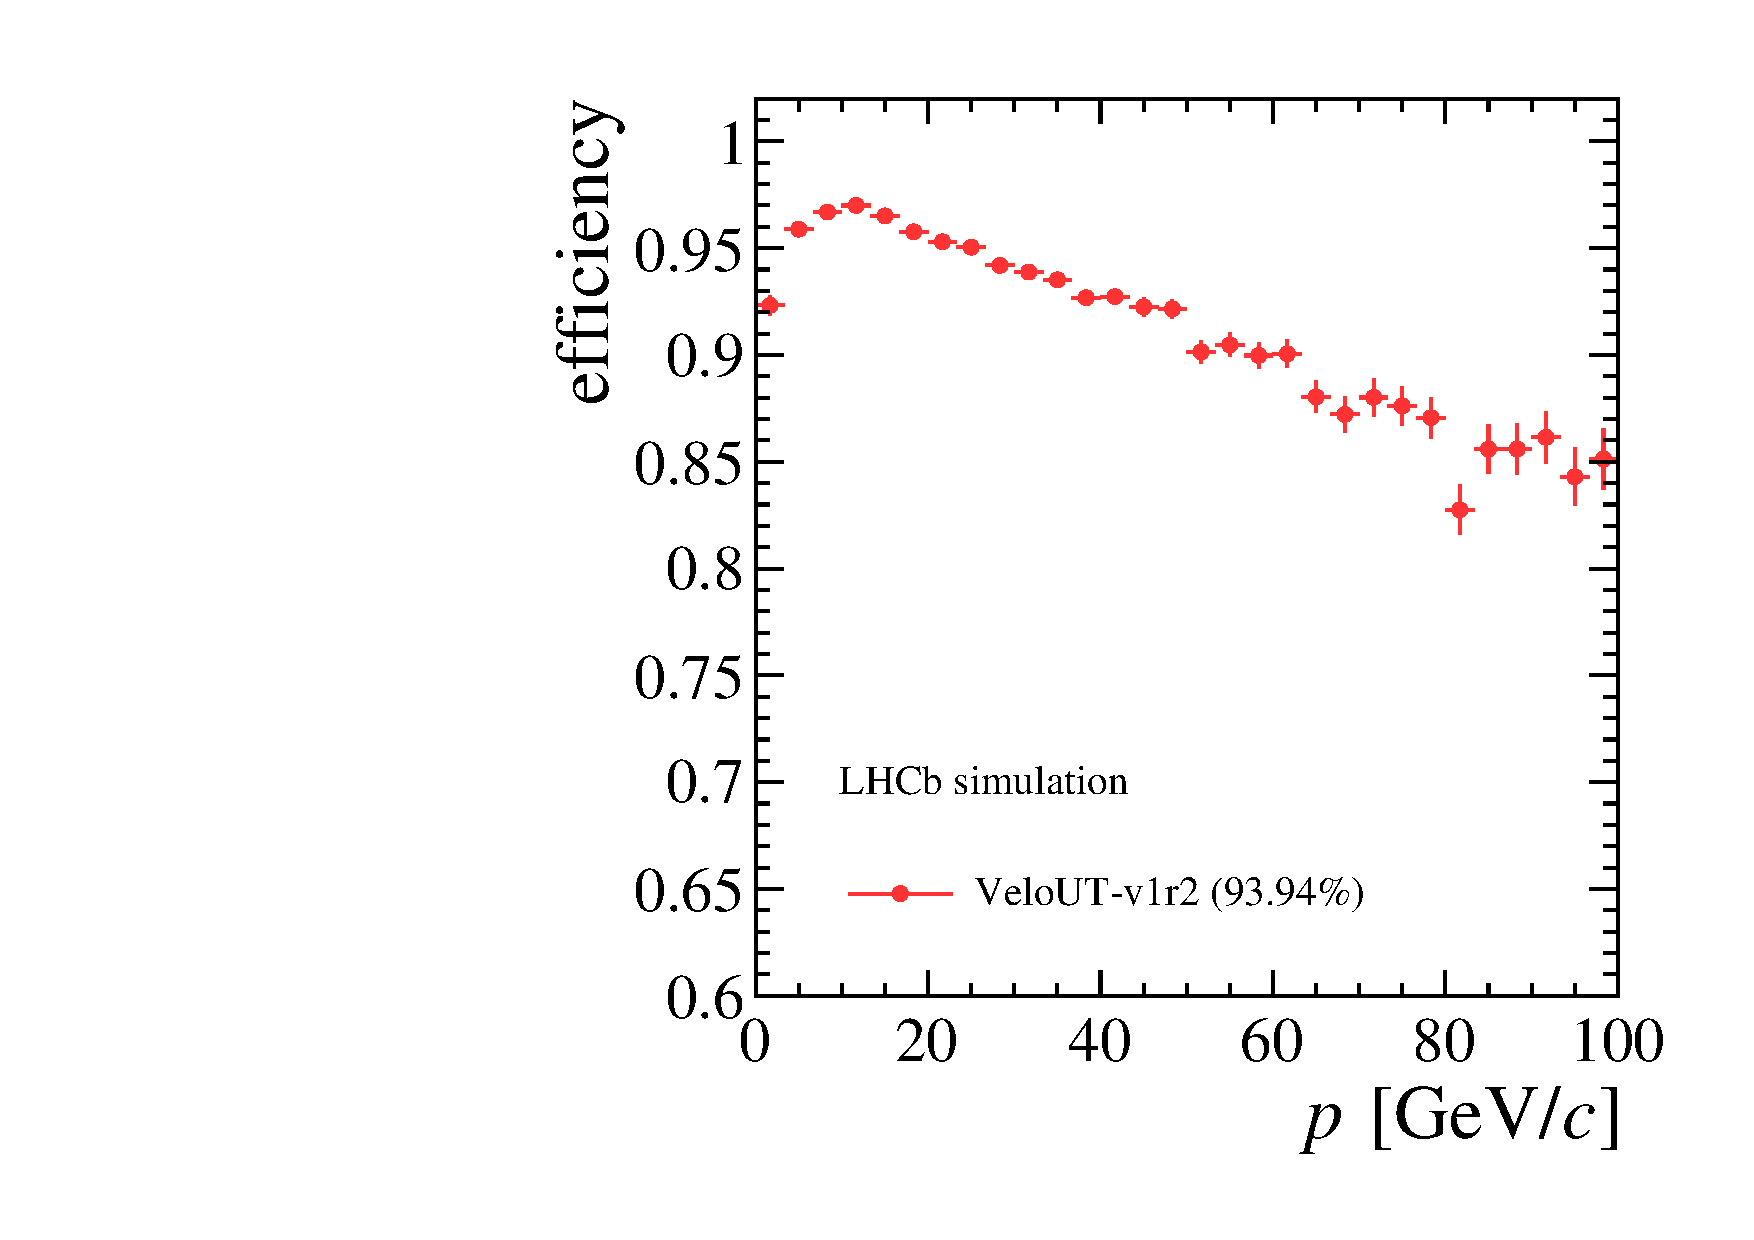
\includegraphics[width=0.45\textwidth]{figs/upstream-tracking-upgrade/eff_p_v1r2.pdf}
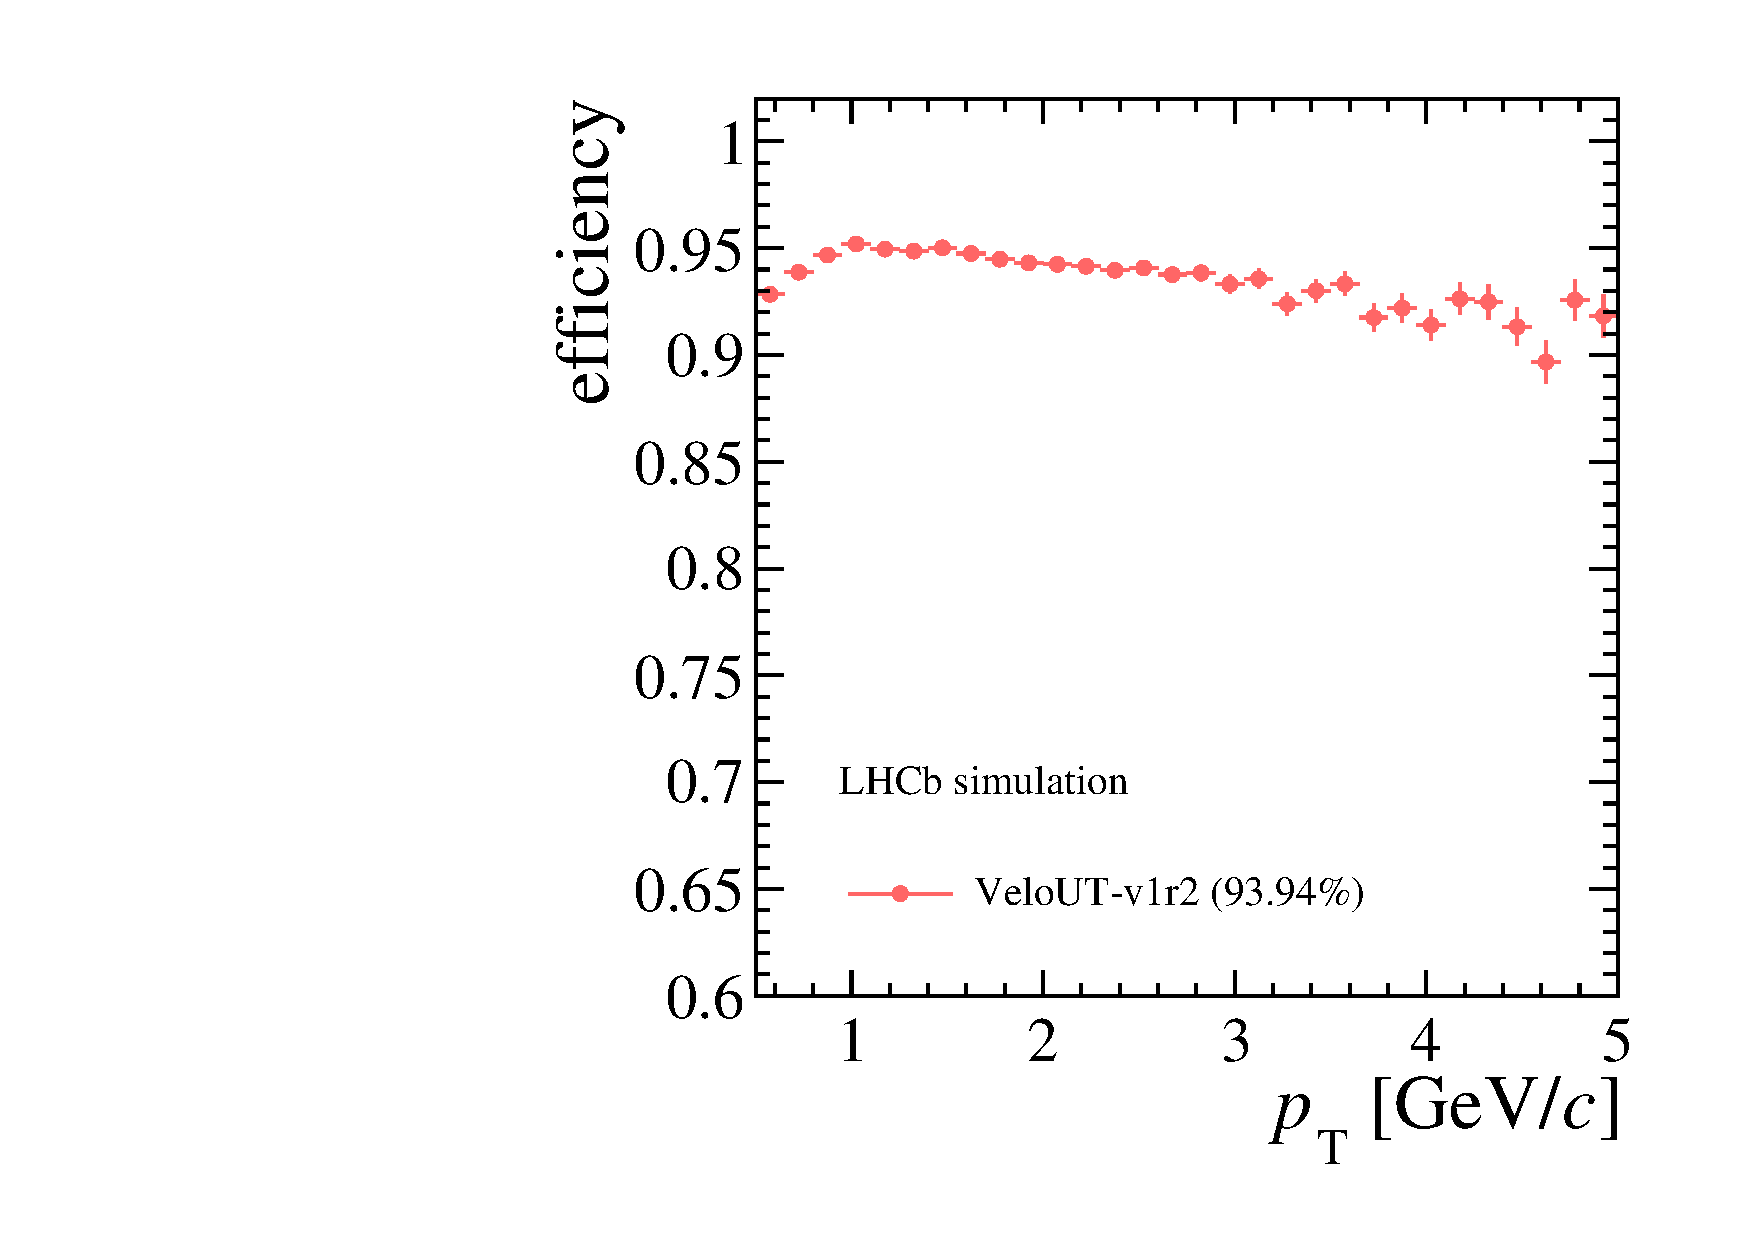
\includegraphics[width=0.45\textwidth]{figs/upstream-tracking-upgrade/eff_pt_v1r2.pdf}
\caption{The reconstruction efficiency as a function of \ptot and \pt for the initial version (\texttt{v1r2}) of the \velout algorithm. There is a clear drop in the reconstruction efficiency as a function of \ptot.}
\label{fig:eff_velout_v1r2}
\end{figure}

\begin{figure}[!tb]
\centering
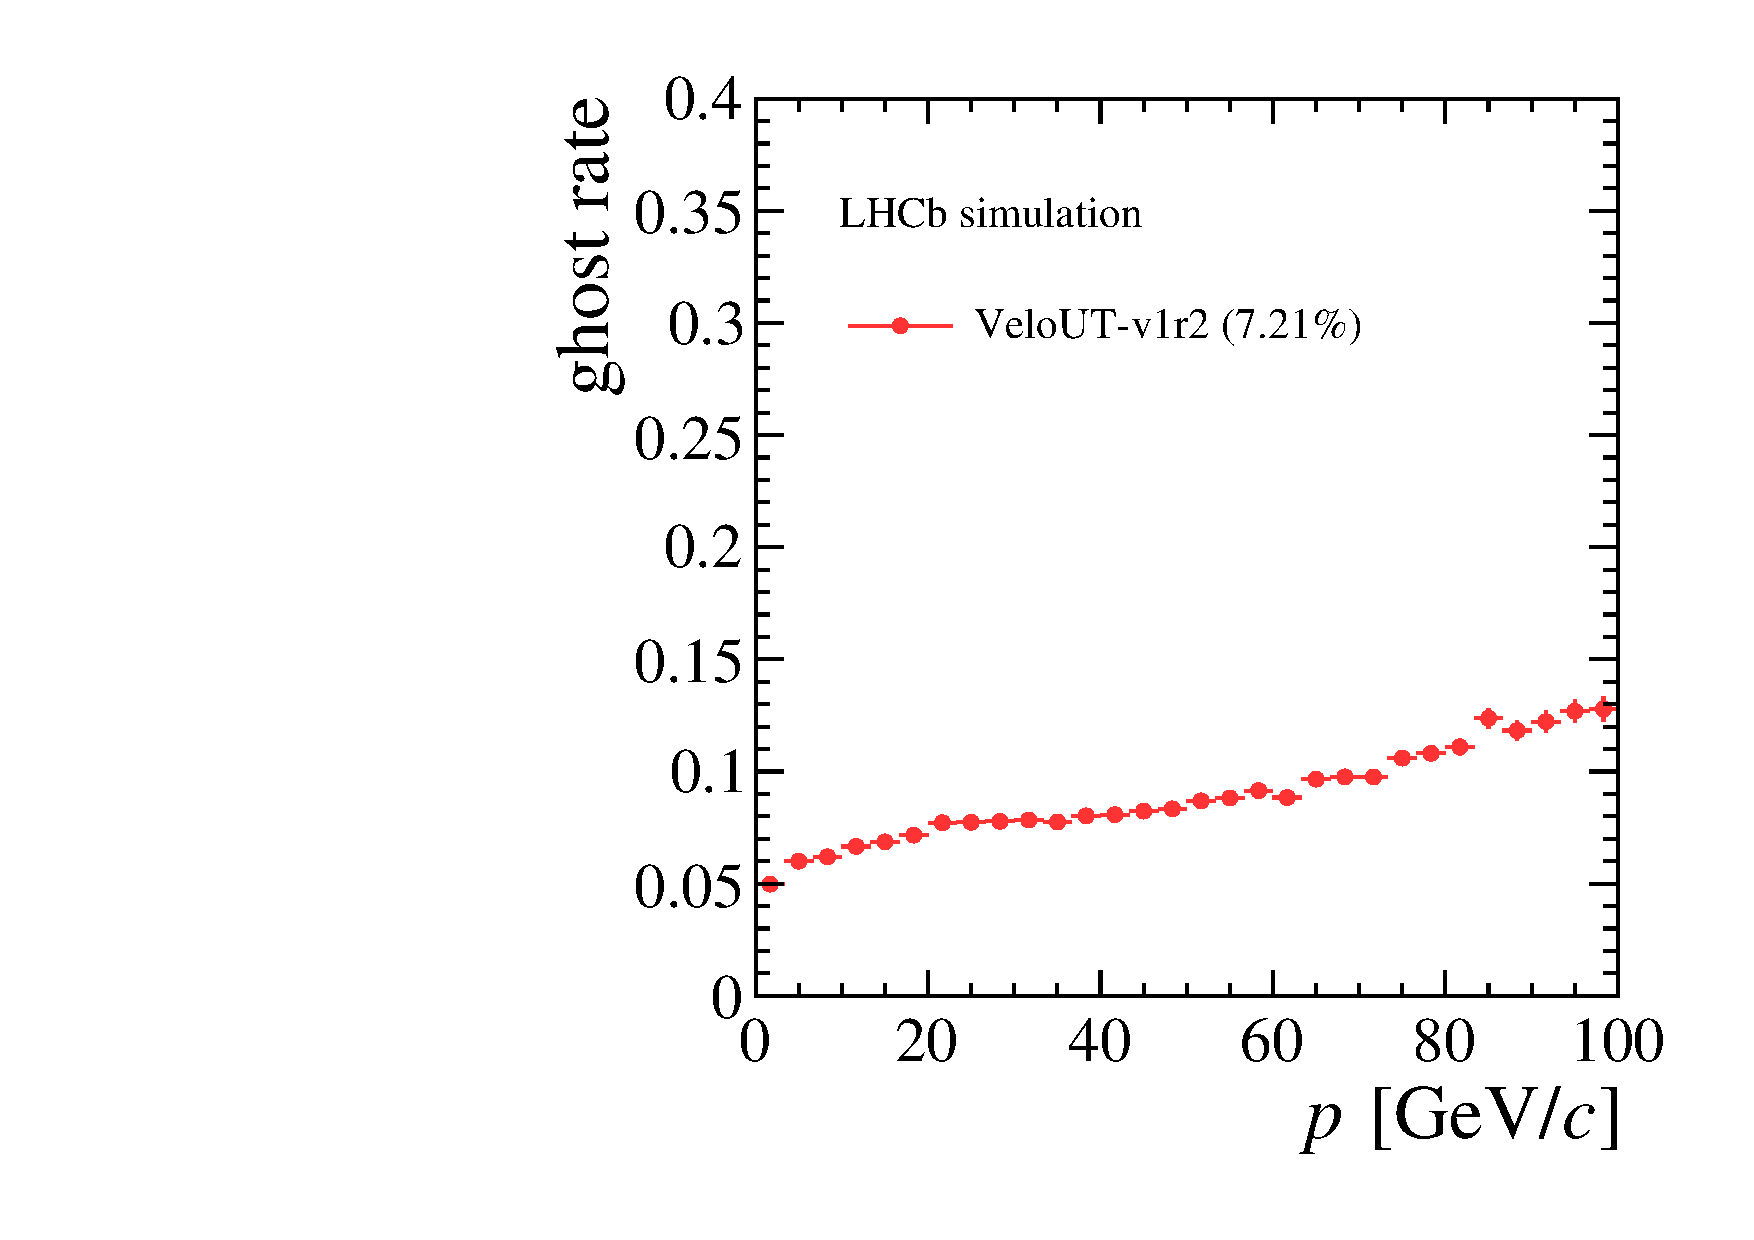
\includegraphics[width=0.45\textwidth]{figs/upstream-tracking-upgrade/gr_p_v1r2.pdf}
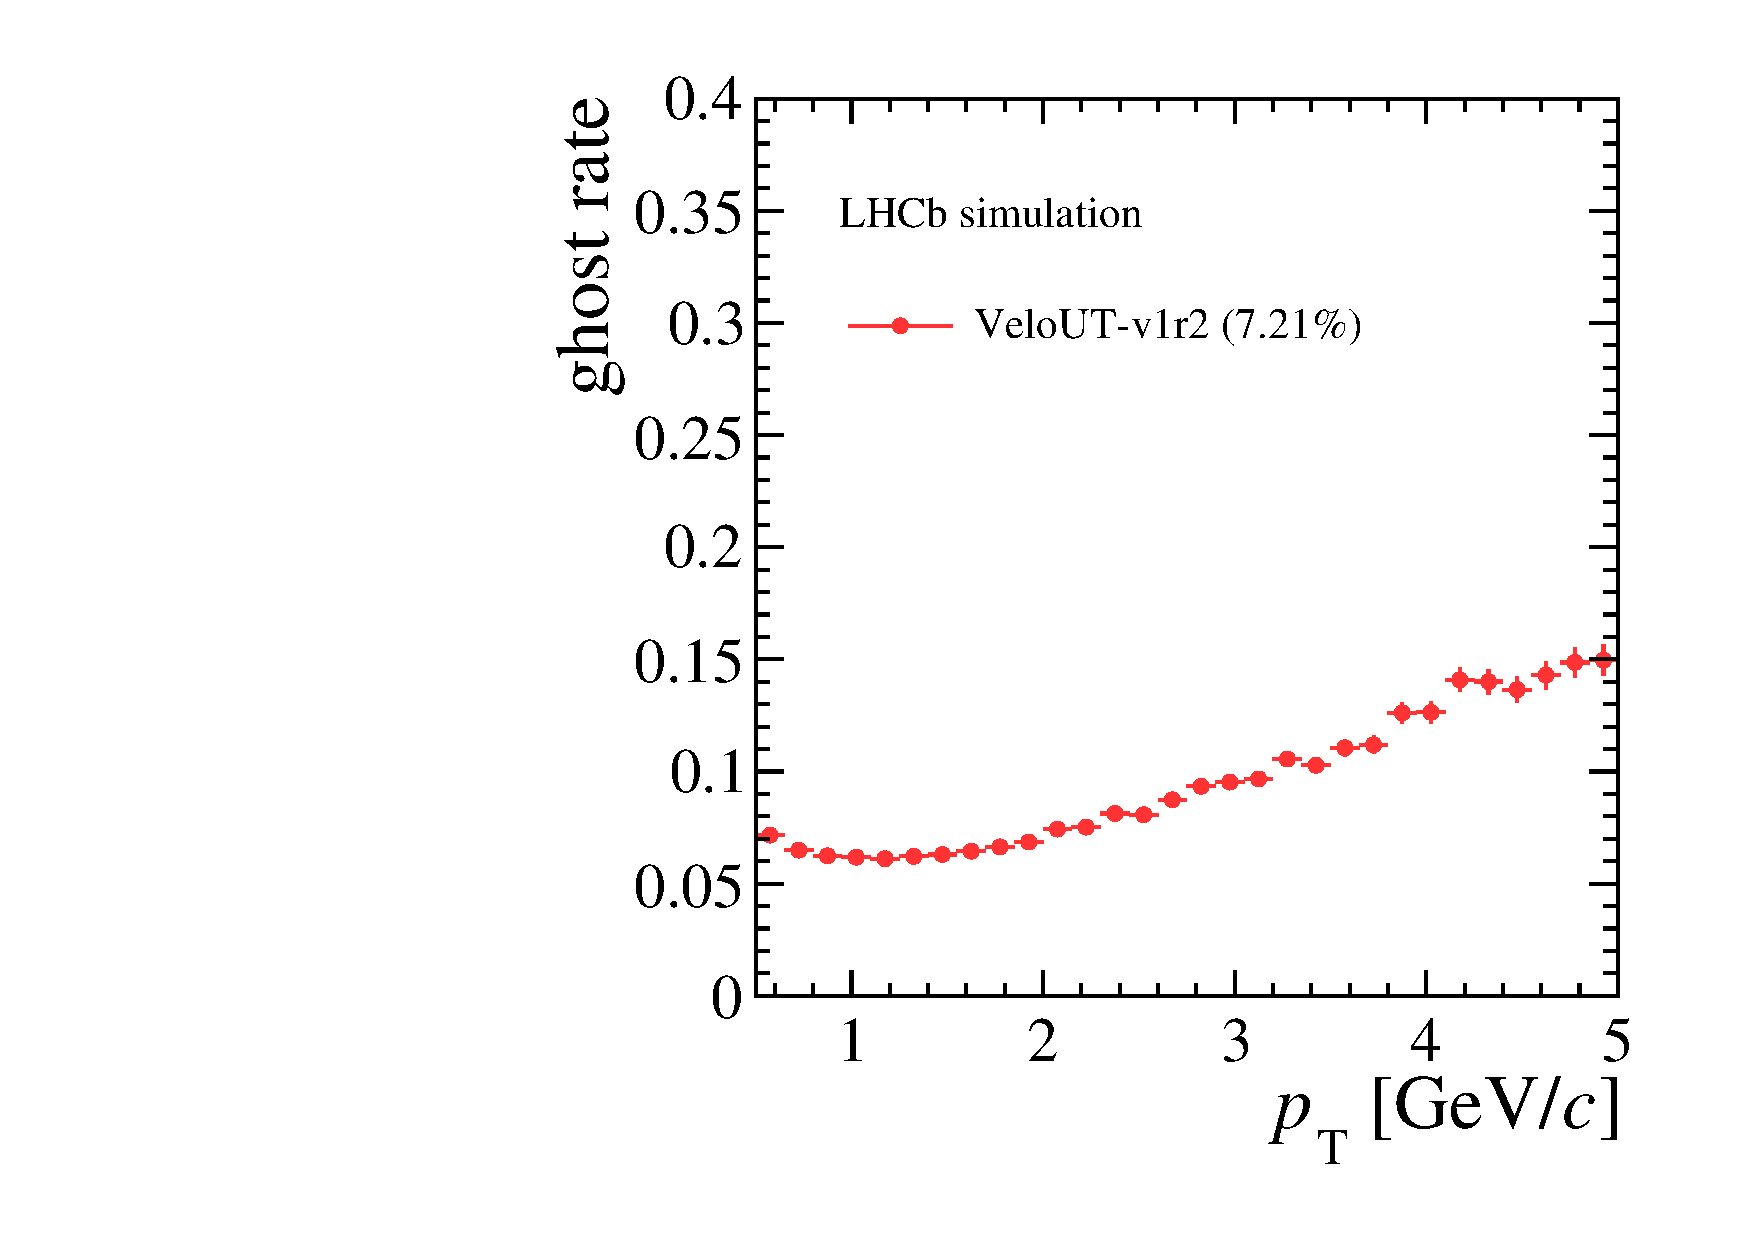
\includegraphics[width=0.45\textwidth]{figs/upstream-tracking-upgrade/gr_pt_v1r2.pdf}
\caption{The ghost rate as a function of \ptot and \pt for the initial version (\texttt{v1r2}) of the \velout algorithm.}
\label{fig:gr_velout_v1r2}
\end{figure}

\subsection{Improvements}

In order to meet the requirements of the software trigger a number of improvements were made to the \velout algorithm. This involved numerous \cpp optimisations as well as changes to the logic. The three changes which had the largest effect are described in detail below.

\subsubsection{Binary searches}

Previously, the UT hits were sorted by detector regions within layers. This meant that for each layer, each detector region was looped over and if it was compatible with the extrapolated \velo track each hit within that region was looped over. In the new version, the hits in each layer are sorted by their $x$ position at $y = 0$. For each layer, a binary search is performed to find the first hit which is within the search window. The hits are then looped over until that requirement is no longer satisfied. The new method greatly reduces the execution time.

\subsubsection{Hit clustering}

The inital version of the \velout algorithm used a Hough transform based on the distance of the hit from linear extrapolation of the \velo track to find cluster candidates. It required that all hits were located on one side of the extrapolated \velo track in the $x$-$z$ plane. While this is a good assumption for low \ptot tracks, it is not the case for high \ptot tracks. For high \ptot tracks, a significant number have at least one hit on the opposite side of the linearly extrapolated \velo track, as shown in Fig.~\ref{fig:wrong_side_hits}. This caused the track reconstruction efficiency to fall with increasing \ptot.

\begin{figure}[!tb]
\centering
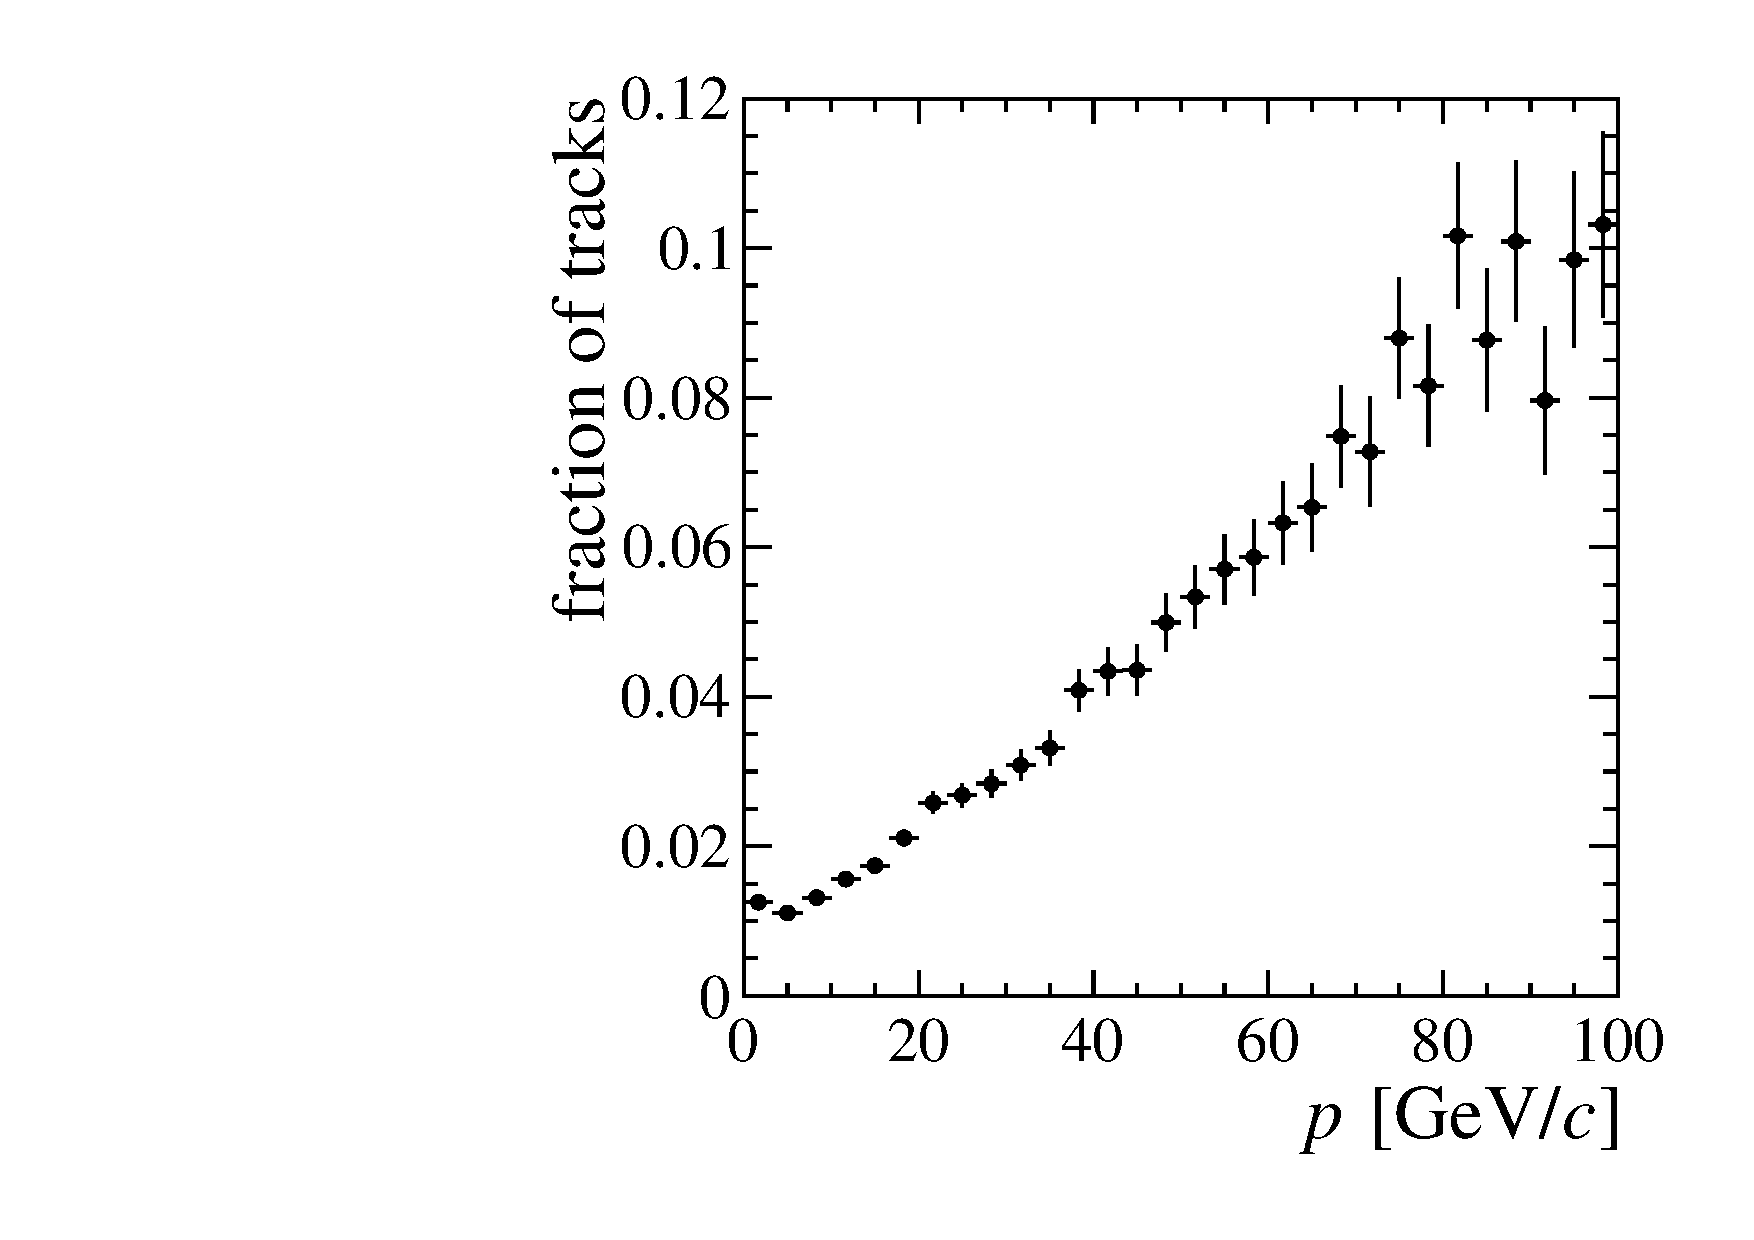
\includegraphics[width=0.45\textwidth]{figs/upstream-tracking-upgrade/wrong_side_hits.pdf}
\caption{The fraction of truth matched tracks with at least one hit on the opposite side of the linearly extrapolated \velo track in the $x$-$z$ plane as a function of \ptot.}
\label{fig:wrong_side_hits}
\end{figure}

A new method for clustering UT hits was developed in order to remedy this flaw and is shown schematically in Fig.~\ref{fig:clustering}. In this new method, UT hits are clustered by first forming doublets (two hits in the same station but in different layers), and then extending those doublets to the opposite station and searching for compatible hits to form triplets or quadruplets. 
 
A doublet is formed by taking one hit in the first layer and another in the second layer. The $x$-slope of the doublet is calculated and if it is below a given threshold the doublet is linearly extrapolated to the third layer where a tolerance window is opened. If there are compatible hits within this window, triplets are formed. For each triplet, the doublet is linearly extrapolated to the fourth layer. A reduced tolerance window is opened and compatible hits are used to form quadruplets. If no quadruplets are formed from any of the triplets, triplets are also searched for with the original doublet and hits in the fourth layer. This process is repeated for every doublet combination.
 
In order to account for missing hits in the UT detector, if no quadruplets have been formed the clustering sequence is run in reverse starting with a doublet in the third and fourth layers.
 
The tolerance window in $x$ around the extrapolated $x$ position of the doublet was tuned in simulation. Using simulated particles and their associated UT hits the difference, $\Delta x$, between the linearly extrapolated $x$ position of a doublet and the $x$ position of an associated hit in a given layer can be found. The distributions used for the tuning are shown in Fig.~\ref{fig:clustering_tolerance}.

\begin{figure}[!tb]
 \begin{center}
\resizebox{0.8\columnwidth}{!}{
  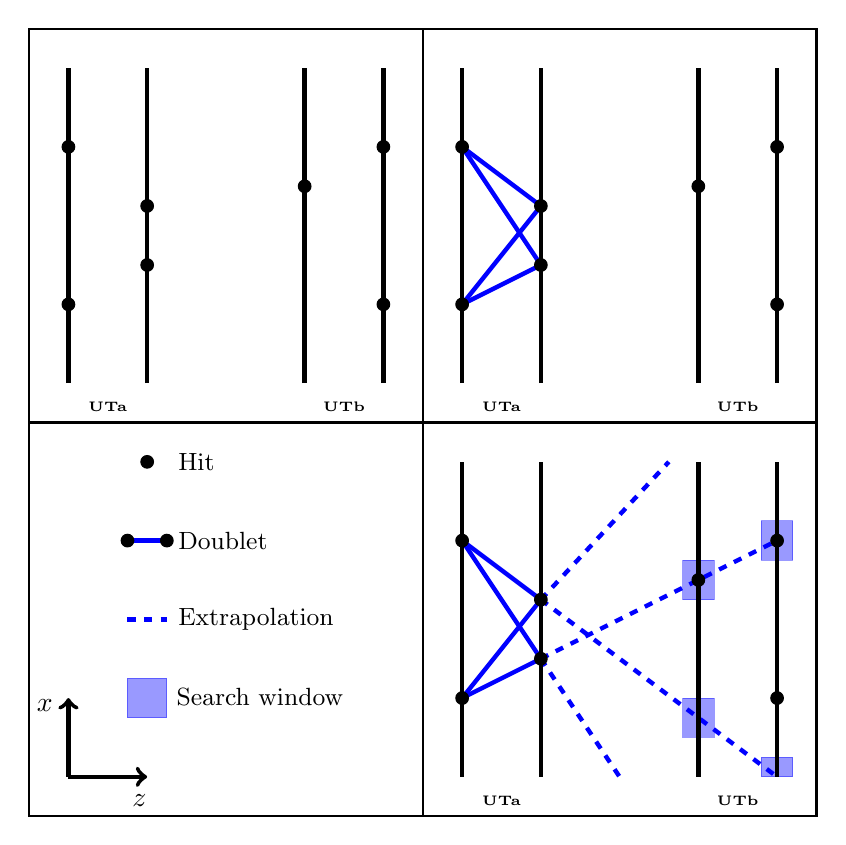
\begin{tikzpicture}
  %\draw[step=1cm,gray,very thin] (0,0) grid (10,10);

  %layout
  \draw[thick] (0,0) rectangle (5,5);
  \draw[thick] (5,0) rectangle (10,5);
  \draw[thick] (0,5) rectangle (5,10);
  \draw[thick] (5,5) rectangle (10,10);

  \draw[thick] (5.0,0.0) -- (5.0,10.0);
  \draw[thick] (0.0,5.0) -- (10.0,5.0);

  %first diagram
  %UT layers
  \draw[ultra thick] (0.5,5.5) -- (0.5,9.5);
  \draw[ultra thick] (1.5,5.5) -- (1.5,9.5);
  \draw[ultra thick] (3.5,5.5) -- (3.5,9.5);
  \draw[ultra thick] (4.5,5.5) -- (4.5,9.5);

  %true hits
  \draw[fill] (0.5,6.5) circle (0.08);
  \draw[fill] (1.5,7.0) circle (0.08);
  \draw[fill] (3.5,8.0) circle (0.08);
  \draw[fill] (4.5,8.5) circle (0.08);

  %fake hits
  \draw[fill] (0.5,8.5) circle (0.08);
  \draw[fill] (1.5,7.75) circle (0.08);
  \draw[fill] (4.5,6.5) circle (0.08);

  %labels
  \node[draw=none] at  (1,5.2){\tiny \bf{UTa}};
  \node[draw=none] at  (4,5.2){\tiny \bf{UTb}};

  %second diagram
  %doublets
  \draw[ultra thick,blue] (5.5,6.5) -- (6.5,7);
  \draw[ultra thick,blue] (5.5,6.5) -- (6.5,7.75);

  \draw[ultra thick,blue] (5.5,8.5) -- (6.5,7);
  \draw[ultra thick,blue] (5.5,8.5) -- (6.5,7.75);

  %UT layers
  \draw[ultra thick] (5.5,5.5) -- (5.5,9.5);
  \draw[ultra thick] (6.5,5.5) -- (6.5,9.5);
  \draw[ultra thick] (8.5,5.5) -- (8.5,9.5);
  \draw[ultra thick] (9.5,5.5) -- (9.5,9.5);

  %true hits
  \draw[fill] (5.5,6.5) circle (0.08);
  \draw[fill] (6.5,7.0) circle (0.08);
  \draw[fill] (8.5,8.0) circle (0.08);
  \draw[fill] (9.5,8.5) circle (0.08);

  %fake hits
  \draw[fill] (5.5,8.5) circle (0.08);
  \draw[fill] (6.5,7.75) circle (0.08);
  \draw[fill] (9.5,6.5) circle (0.08);

  %labels
  \node[draw=none] at  (6,5.2){\tiny \bf{UTa}};
  \node[draw=none] at  (9,5.2){\tiny \bf{UTb}};

  %third diagram
  %doublets
  \draw[ultra thick,blue] (5.5,1.5) -- (6.5,2.0);
  \draw[ultra thick,blue] (5.5,1.5) -- (6.5,2.75);

  \draw[ultra thick,blue] (5.5,3.5) -- (6.5,2.0);
  \draw[ultra thick,blue] (5.5,3.5) -- (6.5,2.75);

  %extrapolations
  %true
  \draw[ultra thick,blue,dashed] (6.5,2.0) -- (9.5,3.5);
  %fake
  \draw[ultra thick,blue,dashed] (6.5,2.0) -- (7.5,0.5);
  \draw[ultra thick,blue,dashed] (6.5,2.75) -- (8.125,4.5);
  \draw[ultra thick,blue,dashed] (6.5,2.75) -- (9.5,0.5);

  %search windows
  %true
  \draw[fill,blue,opacity=0.4] (8.3,2.75) rectangle (8.7,3.25);
  \draw[fill,blue,opacity=0.4] (9.3,3.25) rectangle (9.7,3.75);
  %fake
  \draw[fill,blue,opacity=0.4] (8.3,1.0) rectangle (8.7,1.50);
  \draw[fill,blue,opacity=0.4] (9.3,0.5) rectangle (9.7,0.75);

  %UT layers
  \draw[ultra thick] (5.5,0.5) -- (5.5,4.5);
  \draw[ultra thick] (6.5,0.5) -- (6.5,4.5);
  \draw[ultra thick] (8.5,0.5) -- (8.5,4.5);
  \draw[ultra thick] (9.5,0.5) -- (9.5,4.5);

  %true hits
  \draw[fill] (5.5,1.5) circle (0.08);
  \draw[fill] (6.5,2.0) circle (0.08);
  \draw[fill] (8.5,3.0) circle (0.08);
  \draw[fill] (9.5,3.5) circle (0.08);

  %fake hits
  \draw[fill] (5.5,3.5) circle (0.08);
  \draw[fill] (6.5,2.75) circle (0.08);
  \draw[fill] (9.5,1.5) circle (0.08);

  %labels
  \node[draw=none] at  (6,0.2){\tiny \bf{UTa}};
  \node[draw=none] at  (9,0.2){\tiny \bf{UTb}};

  %legend
  \draw[ultra thick, white] (1.25,4.5) -- (1.75,4.5)  node[anchor=west] {\small \textcolor{black}{Hit}};
  \draw[fill] (1.5,4.5) circle (0.08);

  \draw[ultra thick, blue] (1.25,3.5) -- (1.75,3.5)  node[anchor=west] {\small \textcolor{black}{Doublet}};
  \draw[fill] (1.25,3.5) circle (0.08);
  \draw[fill] (1.75,3.5) circle (0.08);

  \draw[ultra thick, blue,dashed] (1.25,2.5) -- (1.75,2.5) node[anchor=west] {\small \textcolor{black}{Extrapolation}};

  \draw[fill,blue,opacity=0.4,text opacity=1] (1.25,1.25) rectangle (1.75,1.75) node[anchor=north west] {\small \textcolor{black}{Search window}};

  \draw[ultra thick,->] (0.5,0.5) -- (0.5,1.5);
  \draw[ultra thick,->] (0.5,0.5) -- (1.5,0.5);
  \node[draw=none] at  (1.4,0.2){$z$};
  \node[draw=none] at  (0.2,1.4){$x$};

  \end{tikzpicture}
}
   
\caption{A schematic view of the clustering of UT hit candidates. Doublets in the first two layers are formed and then linearly extrapolated to the third and fourth layers to form triplets and quadruplets.}
\label{fig:clustering}
\end{center}
\end{figure}

\begin{figure}[!tb]
\centering
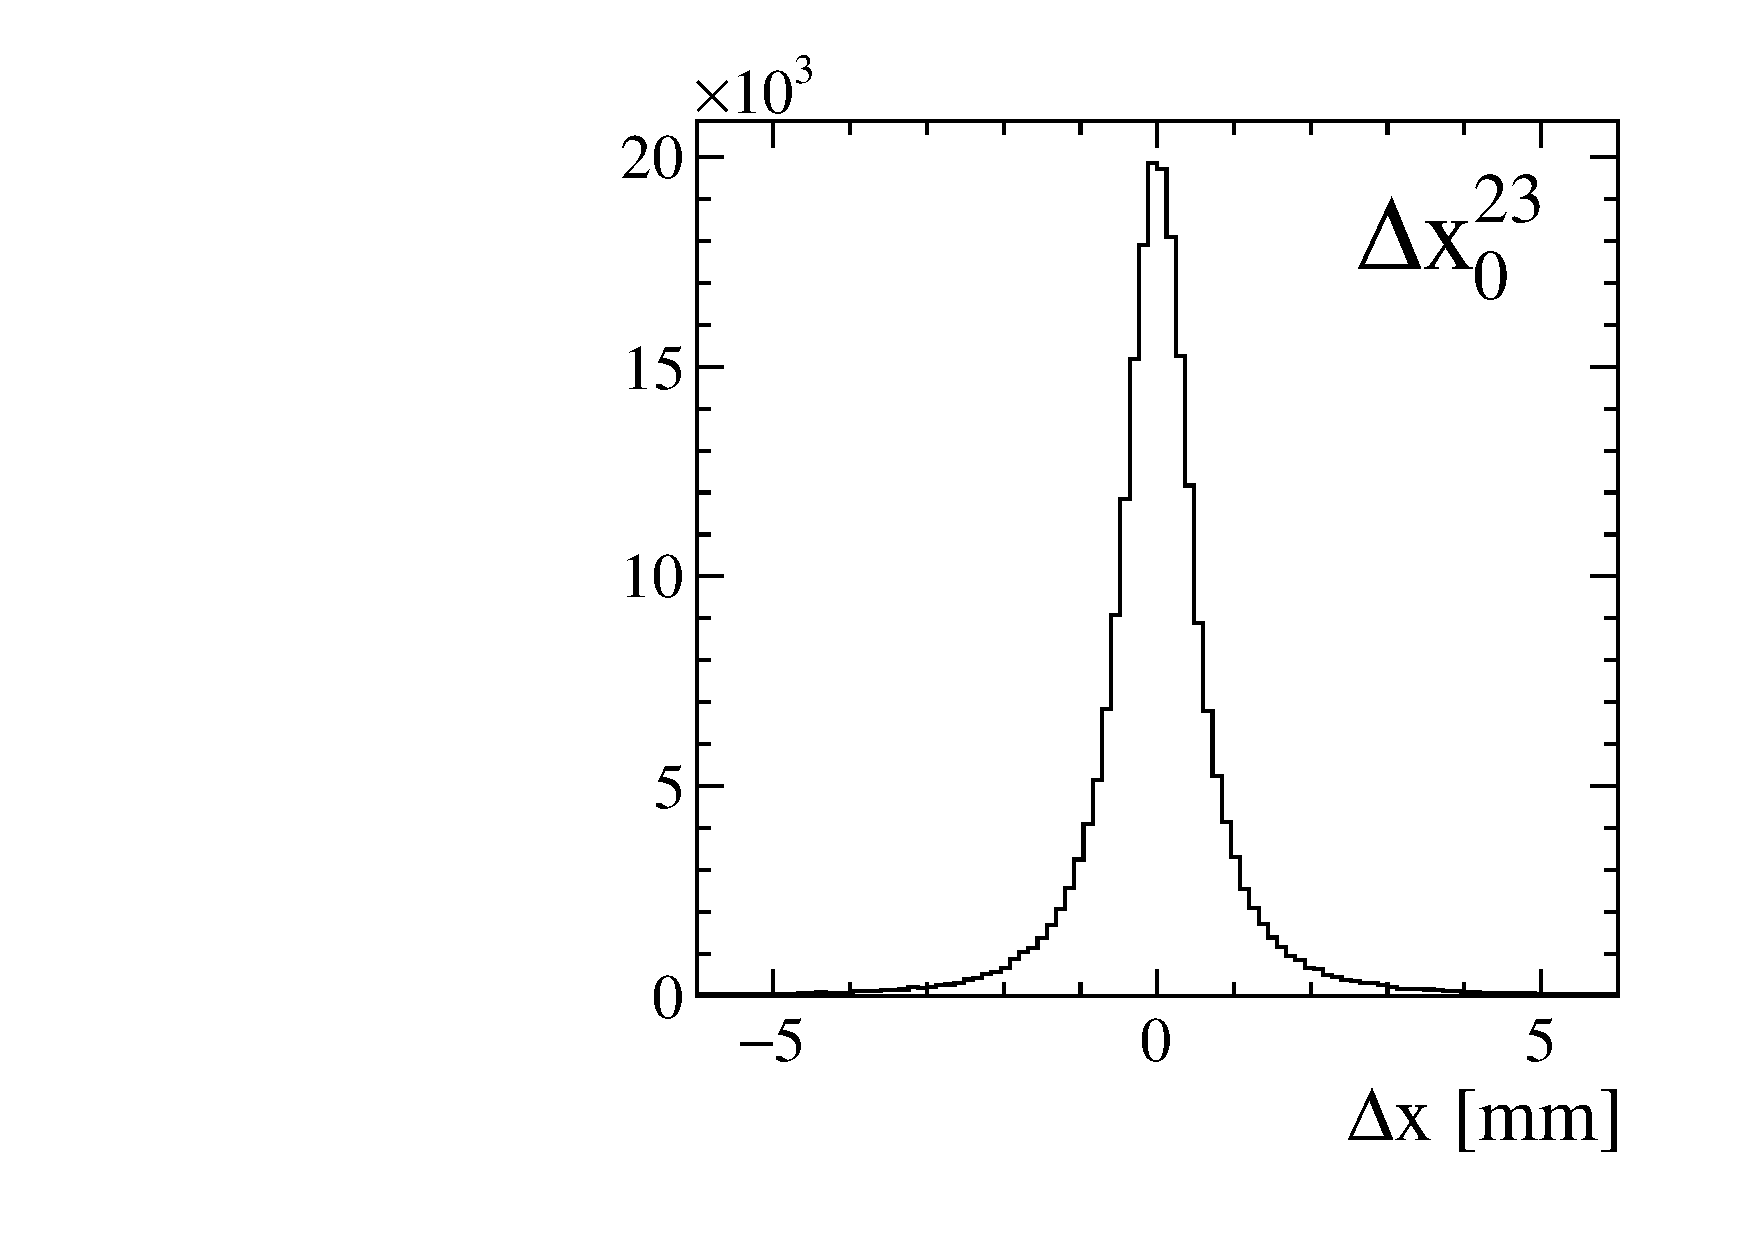
\includegraphics[width=0.32\textwidth]{figs/upstream-tracking-upgrade/dx0.pdf}
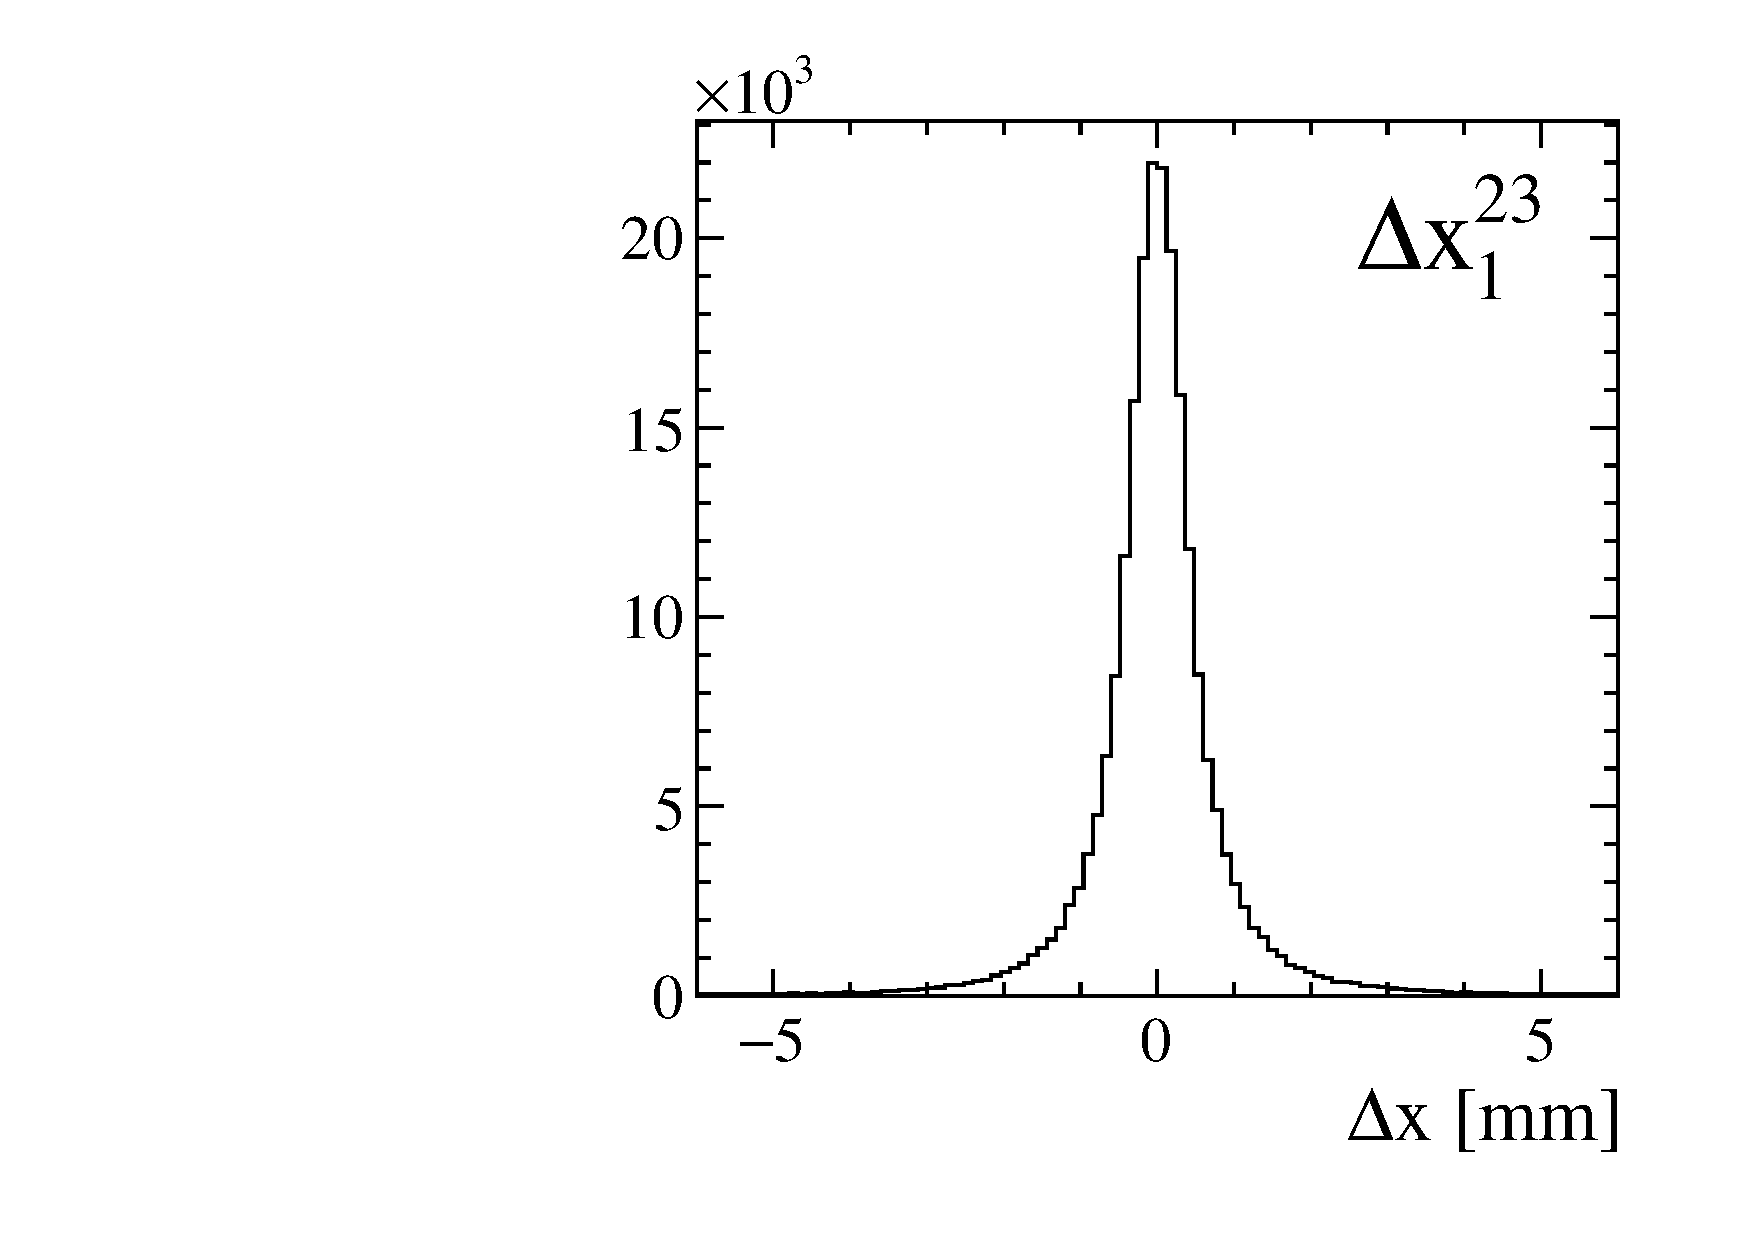
\includegraphics[width=0.32\textwidth]{figs/upstream-tracking-upgrade/dx1.pdf}
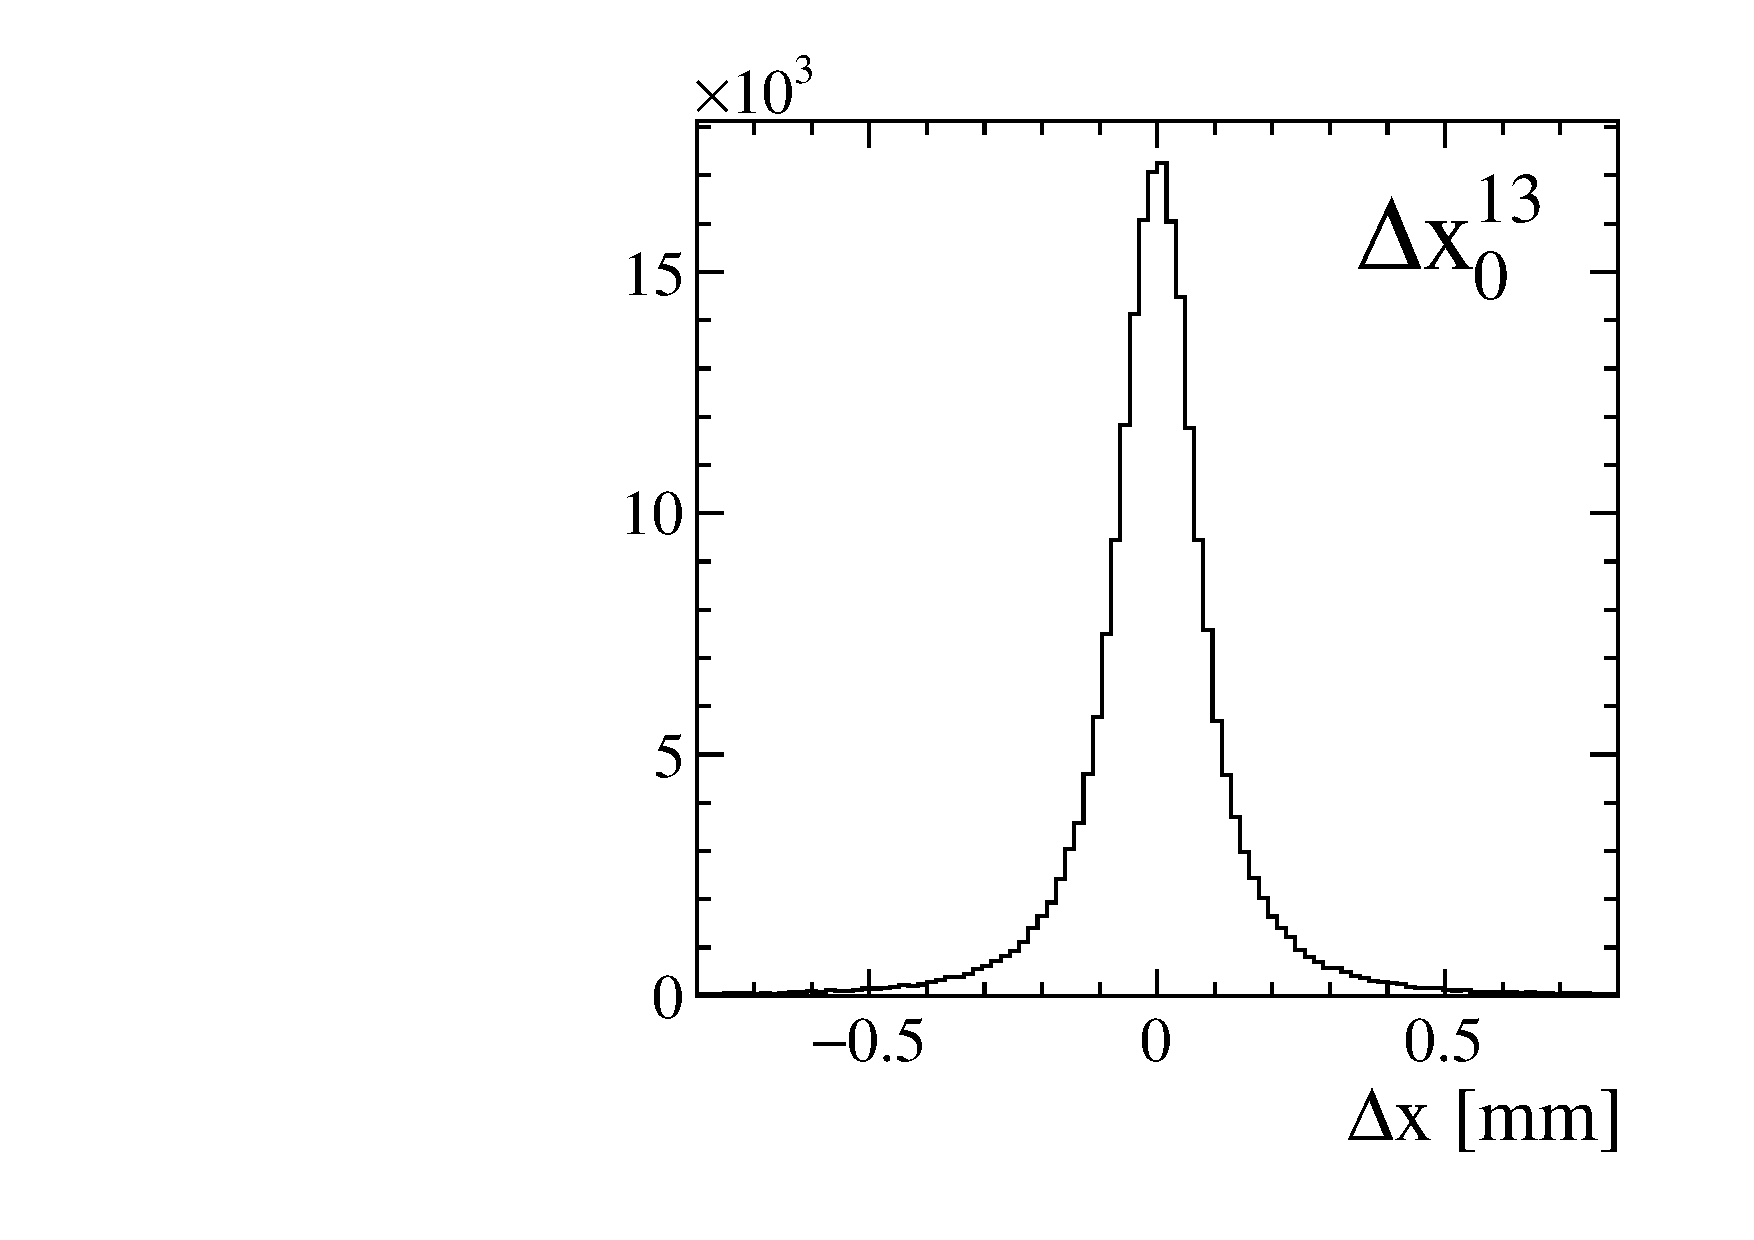
\includegraphics[width=0.32\textwidth]{figs/upstream-tracking-upgrade/dx0b.pdf}
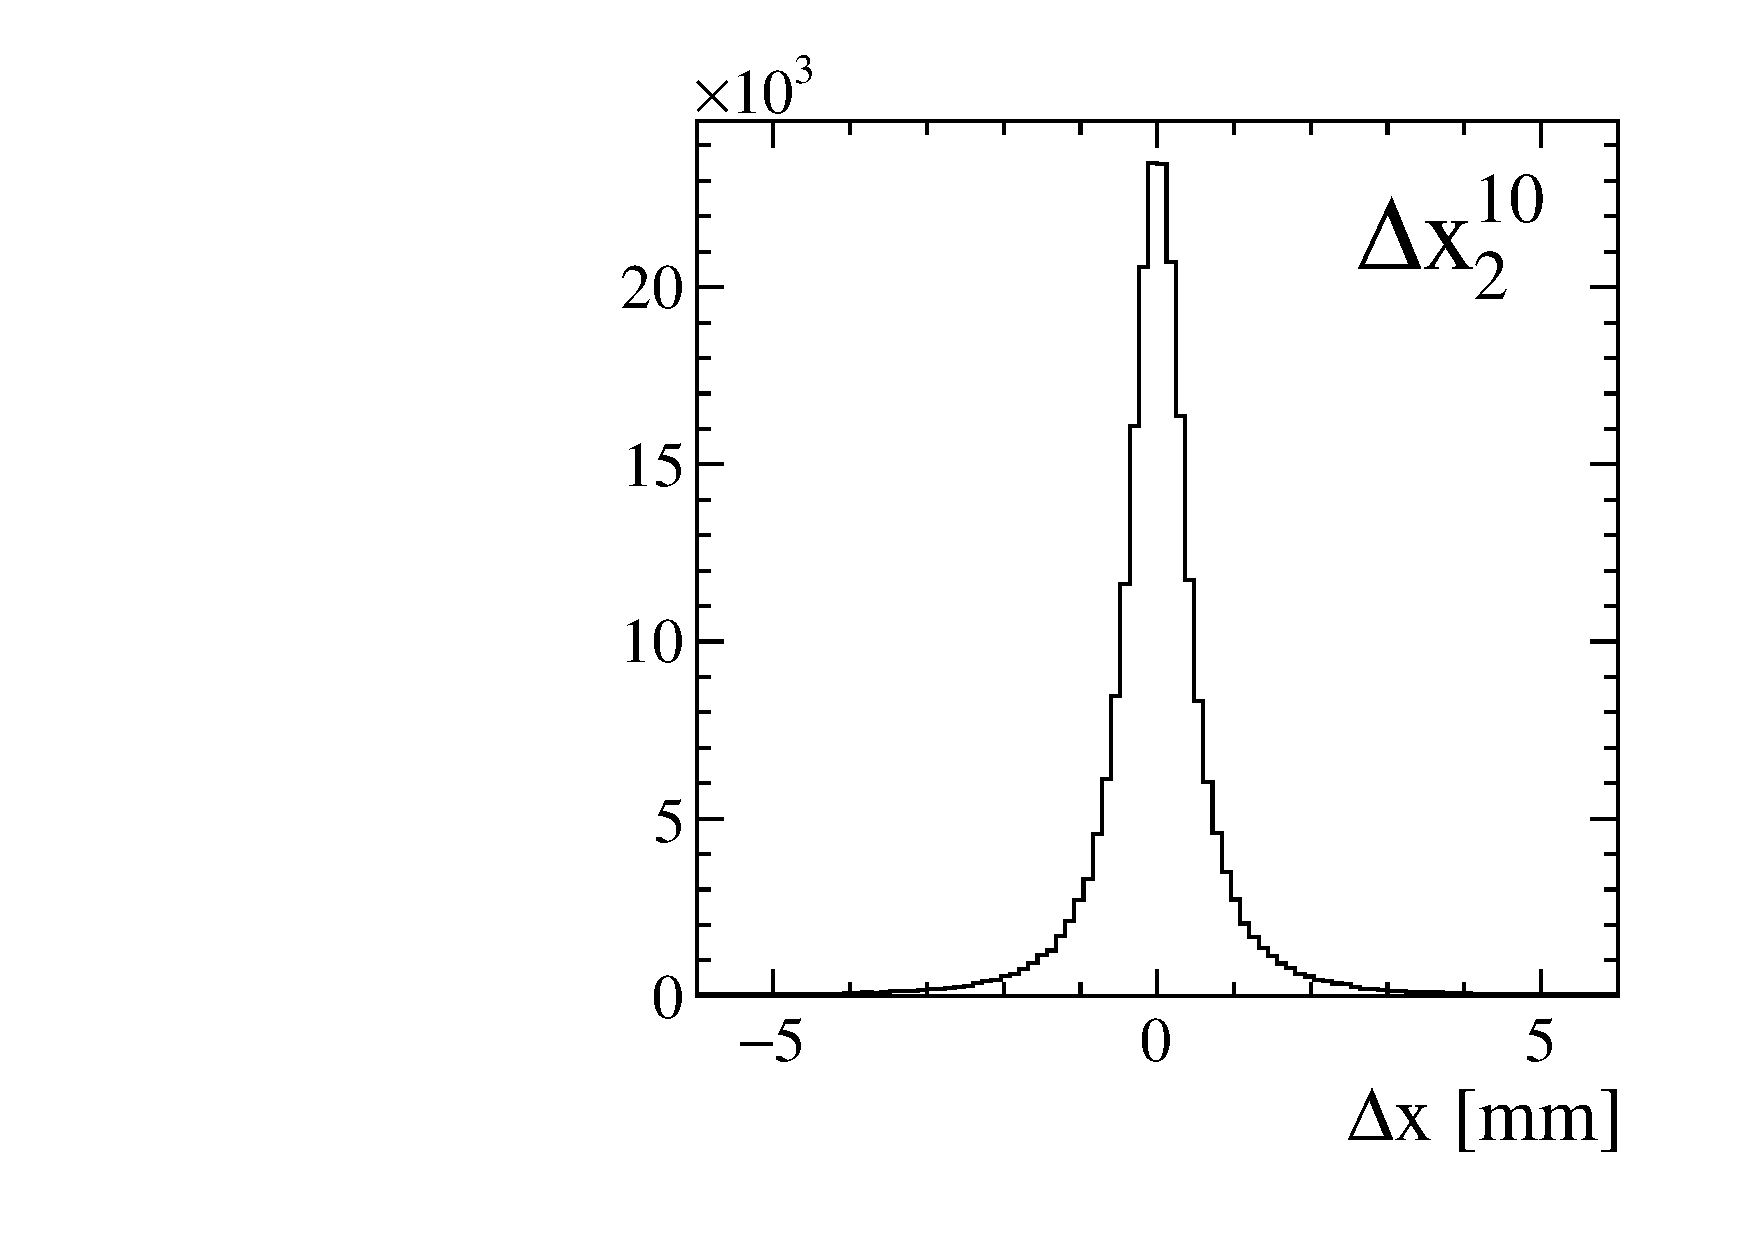
\includegraphics[width=0.32\textwidth]{figs/upstream-tracking-upgrade/dx2.pdf}
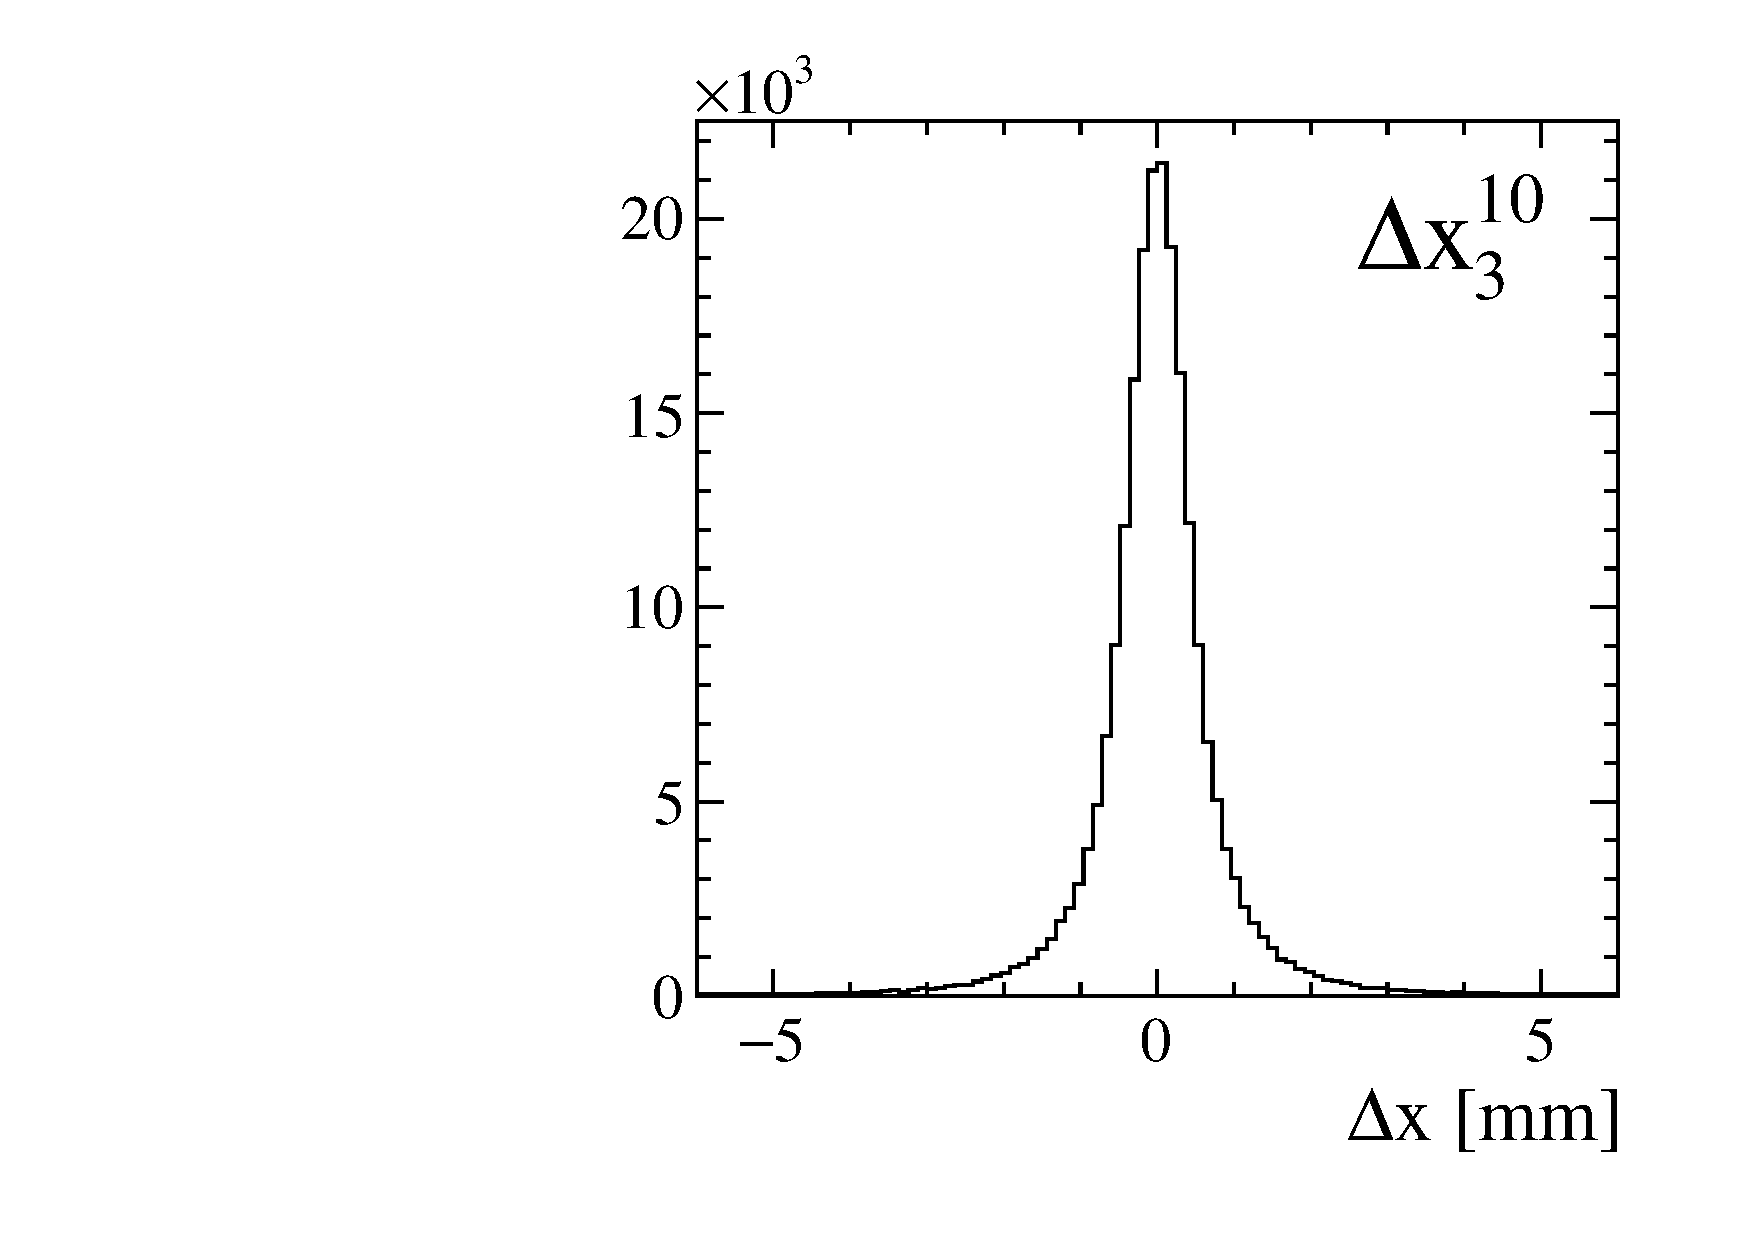
\includegraphics[width=0.32\textwidth]{figs/upstream-tracking-upgrade/dx3.pdf}
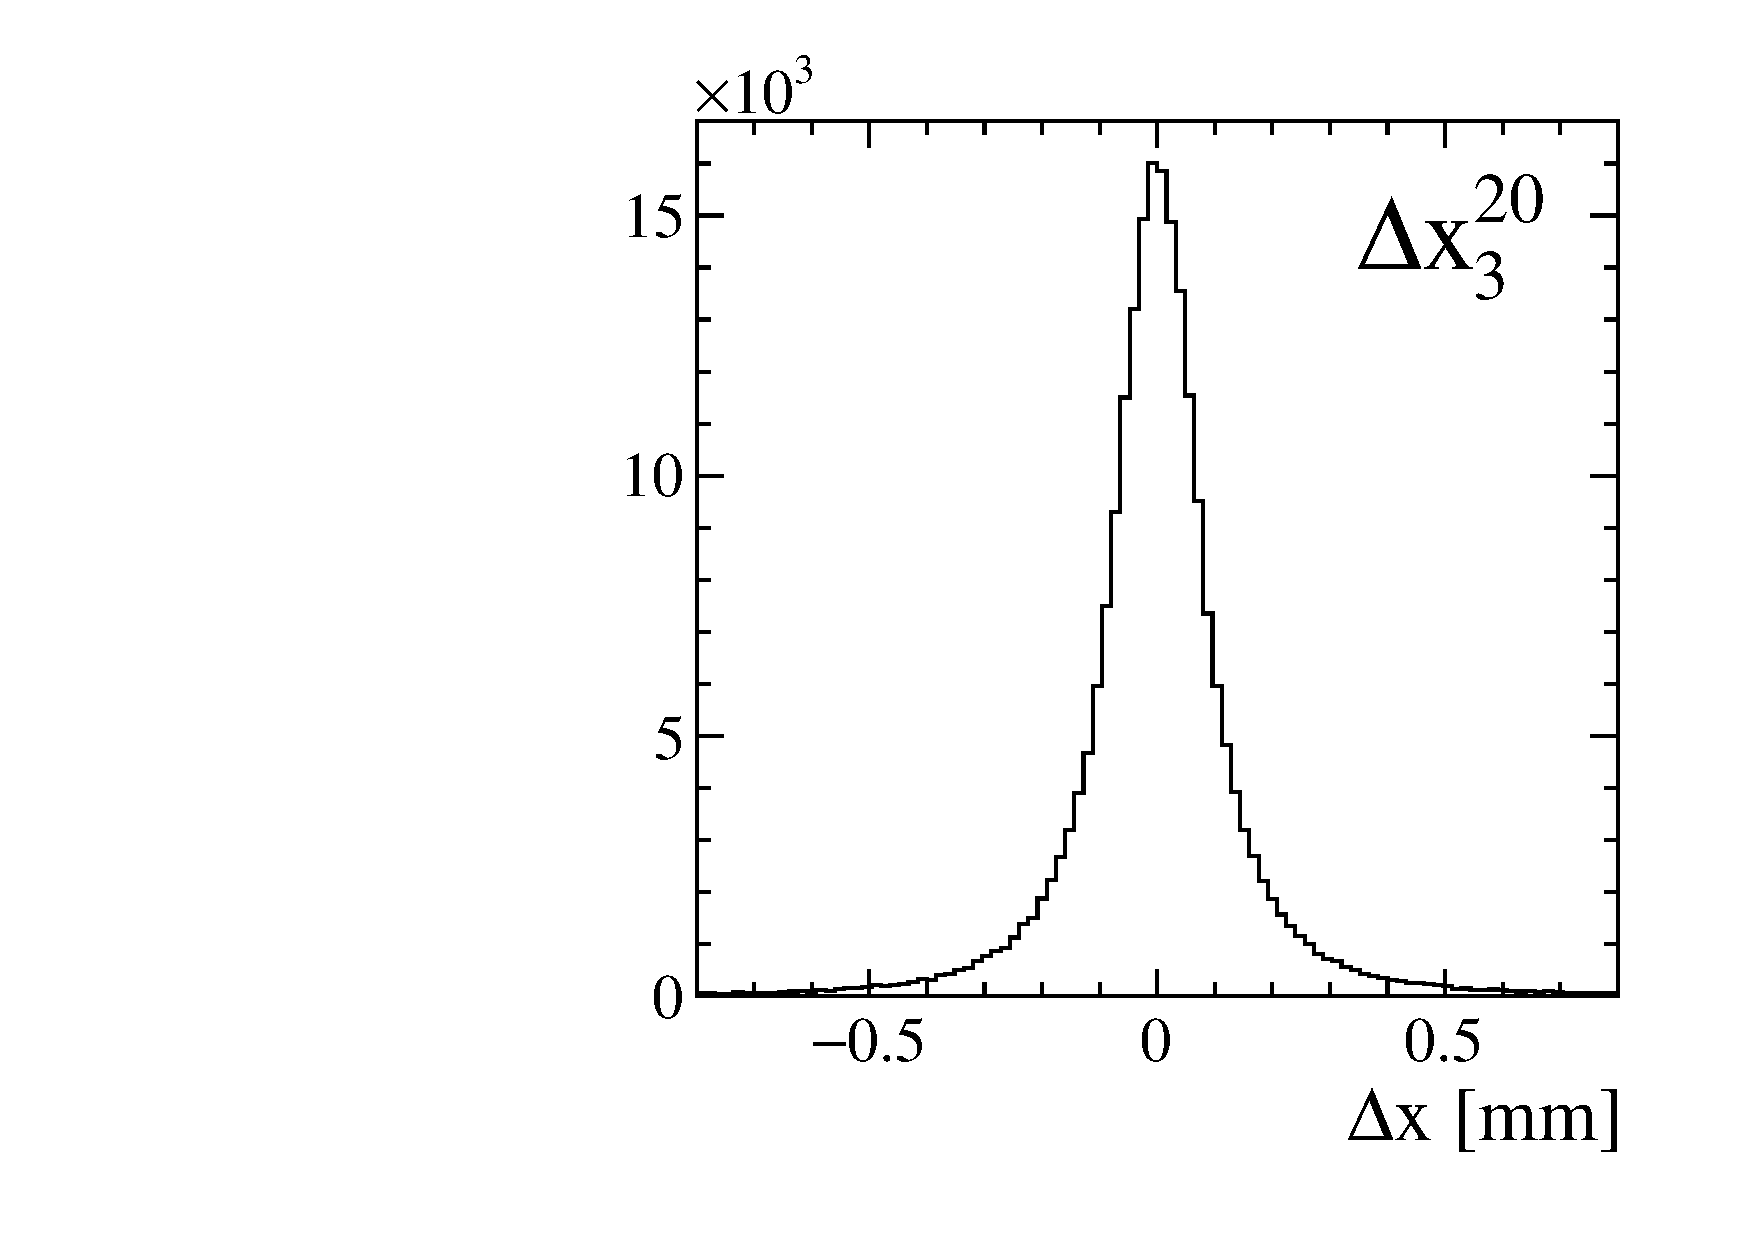
\includegraphics[width=0.32\textwidth]{figs/upstream-tracking-upgrade/dx3b.pdf}
\caption{The difference $\Delta x_{c}^{ab}$ between the linearly extrapolated $x$ position of a doublet and the $x$ position of an associated hit in a given layer where $a$ and $b$ denote the two layers from which the slope has been calculated and $c$ denotes the layer to which the extrapolation is being performed.}
\label{fig:clustering_tolerance}
\end{figure}


\subsubsection{Track fit}

The initial version of the \velout algorithm fitted each of the \velout tracks with a Kalman filter, described in Sec.~\ref{sec:track:fit}, in order to obtain the most accurate estimates of track parameters along with their corresponding covariances. This was very costly in terms of execution time and did not provided any significant improvement to the momentum or charge estimation. The Kalman filter was removed and the momentum and charge information taken from the simplified fit described in Sec.~\ref{sec:track:algos:upstream}, leading to a vast improvement in the execution time.

\subsection{Upgrading to long tracks}

\velout tracks rather than \velo tracks will be used as input to the Forward tracking algorithm in the \lhcb Upgrade. Using the charge and momentum information of the \velout track it is possible to make smarter selections on the input tracks and T-station hits considered by the Forward algorithm. 

A preselection of \pt $>400$\mevc reduces the number of input tracks passed to the Forward tracking by a factor three compared to using \velo tracks. The charge information allows smaller, asymmetric search windows to be opened in the T-stations, reducing the hit multiplicity by a factor two. A small window is also opened on the `wrong' side of the linear extrapolation for high \pt candidates as they are more likely to have been assigned the incorrect charge. The optimised search windows are shown schematically in Fig.~\ref{fig:searchwindow}. These two advancements lead to a greatly reduced execution time and ghost rate of the Forward algorithm. In order to prevent a loss in efficiency due to the central acceptance of the UT, any \velo tracks that are linearly extrapolated within the central hole are passed directly to the Forward tracking algorithm.

\begin{figure}[!tb]
\resizebox{\columnwidth}{!}{
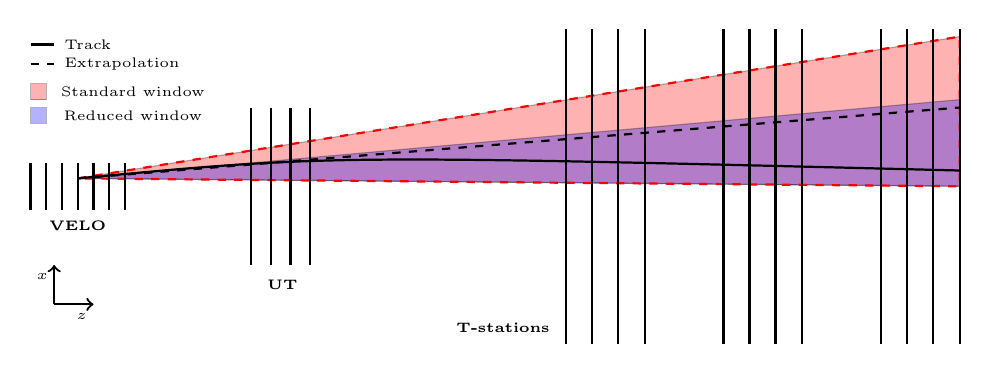
\begin{tikzpicture}
  %\draw[step=1cm,gray,very thin] (0,0) grid (12,4);

  \draw[fill=red,opacity=0.3] (0.8,2.1) -- (12.0,3.9) -- (12.0,2.0)--cycle;
  \draw[fill=blue,opacity=0.3] (0.8,2.1) -- (12.0,3.1) -- (12.0,2.0)--cycle;
  \draw[color=red,dashed,thick] (0.8,2.1) -- (12.0,3.9) -- (12.0,2.0)--cycle;

  %VELO
  \node[draw=none] at  (0.8,1.5){\tiny \bf{VELO}};
  \draw[thick] (0.2,1.7) -- (0.2,2.3);
  \draw[thick] (0.4,1.7) -- (0.4,2.3);
  \draw[thick] (0.6,1.7) -- (0.6,2.3);
  \draw[thick] (0.8,1.7) -- (0.8,2.3);
  \draw[thick] (1.0,1.7) -- (1.0,2.3);
  \draw[thick] (1.2,1.7) -- (1.2,2.3);
  \draw[thick] (1.4,1.7) -- (1.4,2.3);

  %TT
  \node[draw=none] at  (3.4,0.75){\tiny \bf{UT}};
  \draw[thick] (3.0,1.0) -- (3.0,3.0);
  \draw[thick] (3.25,1.0) -- (3.25,3.0);
  \draw[thick] (3.5,1.0) -- (3.5,3.0);
  \draw[thick] (3.75,1.0) -- (3.75,3.0);

  %T
  \node[draw=none] at  (6.2,0.2){\tiny \bf{T-stations}};
  \draw[thick] (7.0,0.0) -- (7.0,4.0);
  \draw[thick] (7.33,0.0) -- (7.33,4.0);
  \draw[thick] (7.66,0.0) -- (7.66,4.0);
  \draw[thick] (8.0,0.0) -- (8.0,4.0);

  \draw[thick] (9.0,0.0) -- (9.0,4.0);
  \draw[thick] (9.33,0.0) -- (9.33,4.0);
  \draw[thick] (9.66,0.0) -- (9.66,4.0);
  \draw[thick] (10.0,0.0) -- (10.0,4.0);

  \draw[thick] (11.0,0.0) -- (11.0,4.0);
  \draw[thick] (11.33,0.0) -- (11.33,4.0);
  \draw[thick] (11.66,0.0) -- (11.66,4.0);
  \draw[thick] (12.0,0.0) -- (12.0,4.0);

  \draw[thick,dashed] (0.8,2.1) -- (12,2+10*0.1);
  \draw[thick] (0.8,2.1) .. controls (4,2.4) .. (12,2.2);

  \draw[thick] (0.2,3.8) -- (0.5,3.8)  node[anchor=west] {\tiny Track};
  \draw[thick,dashed] (0.2,3.55) -- (0.5,3.55)  node[anchor=west] {\tiny Extrapolation};
  \draw[fill=red,opacity=0.3] (0.2,3.1) rectangle (0.4,3.3);
  \draw[fill=blue,opacity=0.3] (0.2,2.8) rectangle (0.4,3.0);

  \node[draw=none] at  (1.5,3.2){\tiny Standard window};
  \node[draw=none] at  (1.5,2.9){\tiny Reduced window};

  \draw[thick,->] (0.5,0.5) -- (0.5,1.0);
  \draw[thick,->] (0.5,0.5) -- (1.0,0.5);
  \node[draw=none] at (0.35,0.85){\tiny $x$};
  \node[draw=none] at (0.85,0.35){\tiny $z$};

\end{tikzpicture}
}

\caption{The search windows opened by the Forward algorithm with and without the charge and momentum information of the VeloUT candidates. The charge information allows smaller, asymmetric search windows to be opened. A small window is also opened on the `wrong' side of the linear extrapolation for high \pt candidates as they are more likely to have been assigned the incorrect charge.}
\label{fig:searchwindow}
\end{figure}

\subsection{Performance}

\subsubsection{\velout}

The track reconstruction efficiency, ghost rate and execution time of the \velout algorithm for both the initial version (\texttt{v1r2}) and the optimised version (\texttt{v2r2}) are shown in Table~\ref{tab:perf_velout_comp}. The track reconstruction efficiency as a function of \ptot and \pt are shown in Fig.~\ref{fig:eff_velout_comp}. The ghost rate as a function of \ptot and \pt are shown in Fig.~\ref{fig:gr_velout_comp}. The optimised version shows large improvements in terms of track reconstruction efficiency and execution time. The increase in reconstruction efficiency is most evident at high \ptot where the initial version shows a negative trend for increasing \ptot. There is also a slight increase in the ghost rate. However, this is of lesser importance as the ghost rate can be further reduced during offline analysis.

\begin{table}[!tb]
\caption{The performances of both the initial version (\texttt{v1r2}) and the optimised version (\texttt{v2r2}) of the \velout algorithm in terms of track reconstruction efficiency, ghost rate and execution time.}
\begin{center}
\begin{tabular}{c|c|c|c}
   \velout & Efficiency [\%] & Ghost rate [\%] & Timing [ms] \\
   \hline
   v1r2  & 93.94  & 7.21  &  27.20  \\
   v2r2  & 98.69  & 8.00 &  \hphantom{0}0.81  \\
 \end{tabular}
 \end{center}
\label{tab:perf_velout_comp}
\end{table}

\begin{figure}[!tb]
\centering
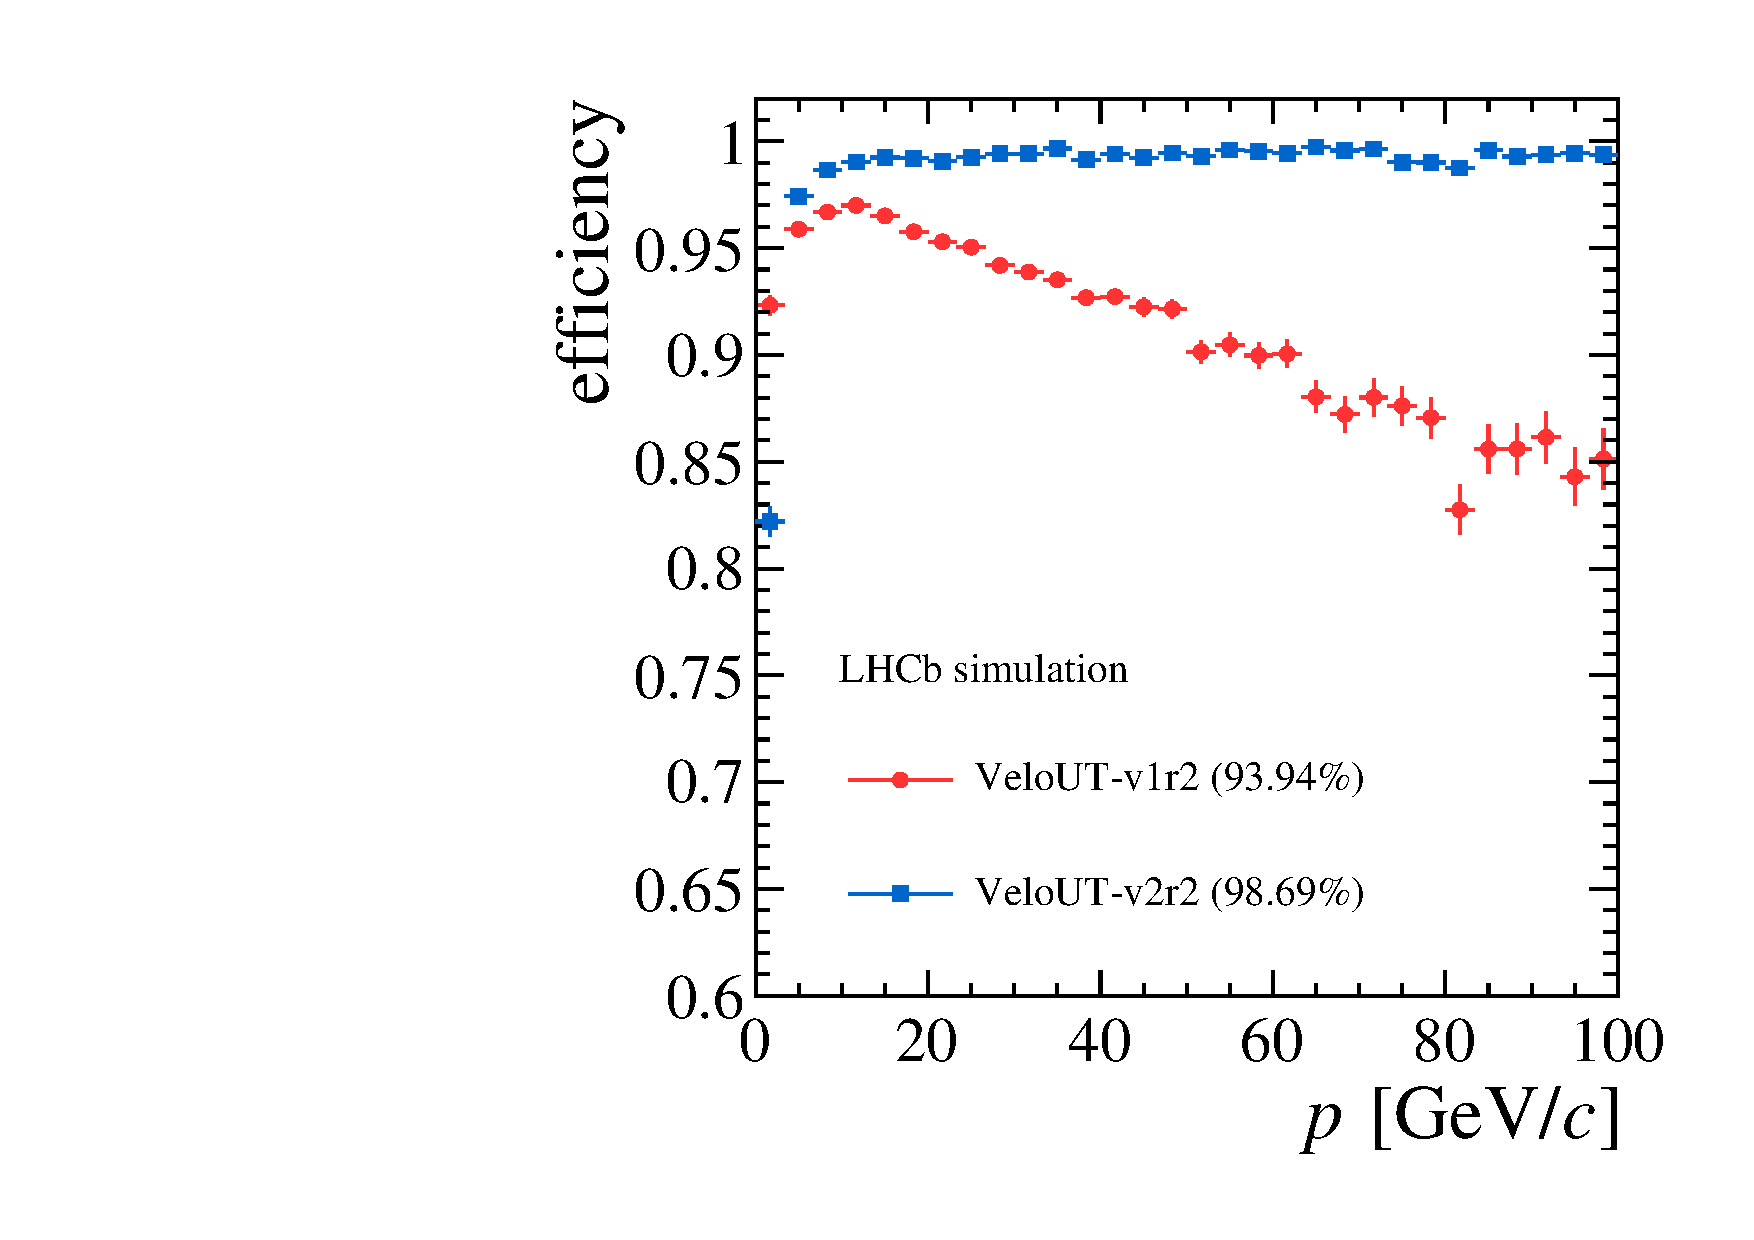
\includegraphics[width=0.45\textwidth]{figs/upstream-tracking-upgrade/eff_p_comp.pdf}
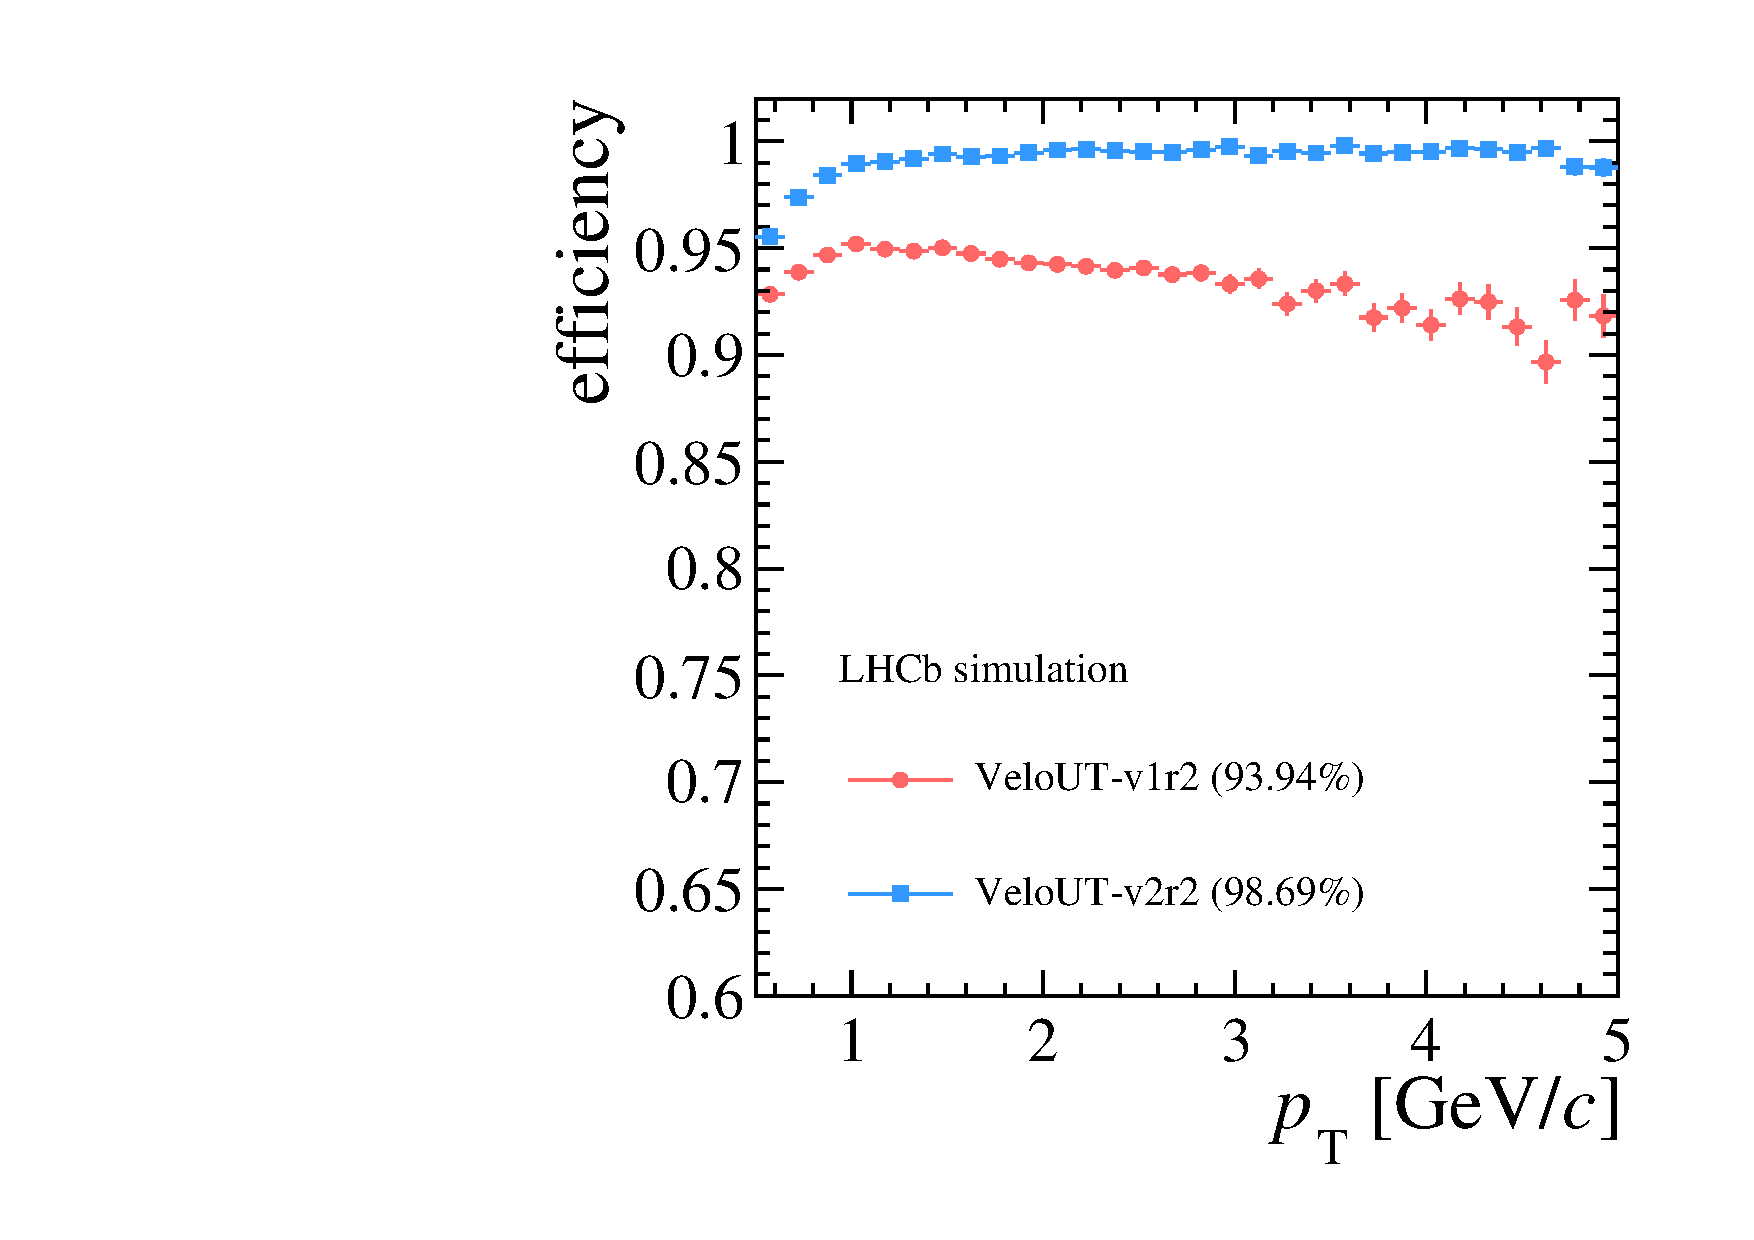
\includegraphics[width=0.45\textwidth]{figs/upstream-tracking-upgrade/eff_pt_comp.pdf}
\caption{The reconstruction efficiency as a function of \ptot and \pt for both the initial version (\texttt{v1r2}) and the optimised version (\texttt{v2r2}) of the \velout algorithm.}
\label{fig:eff_velout_comp}
\end{figure}

\begin{figure}[!tb]
\centering
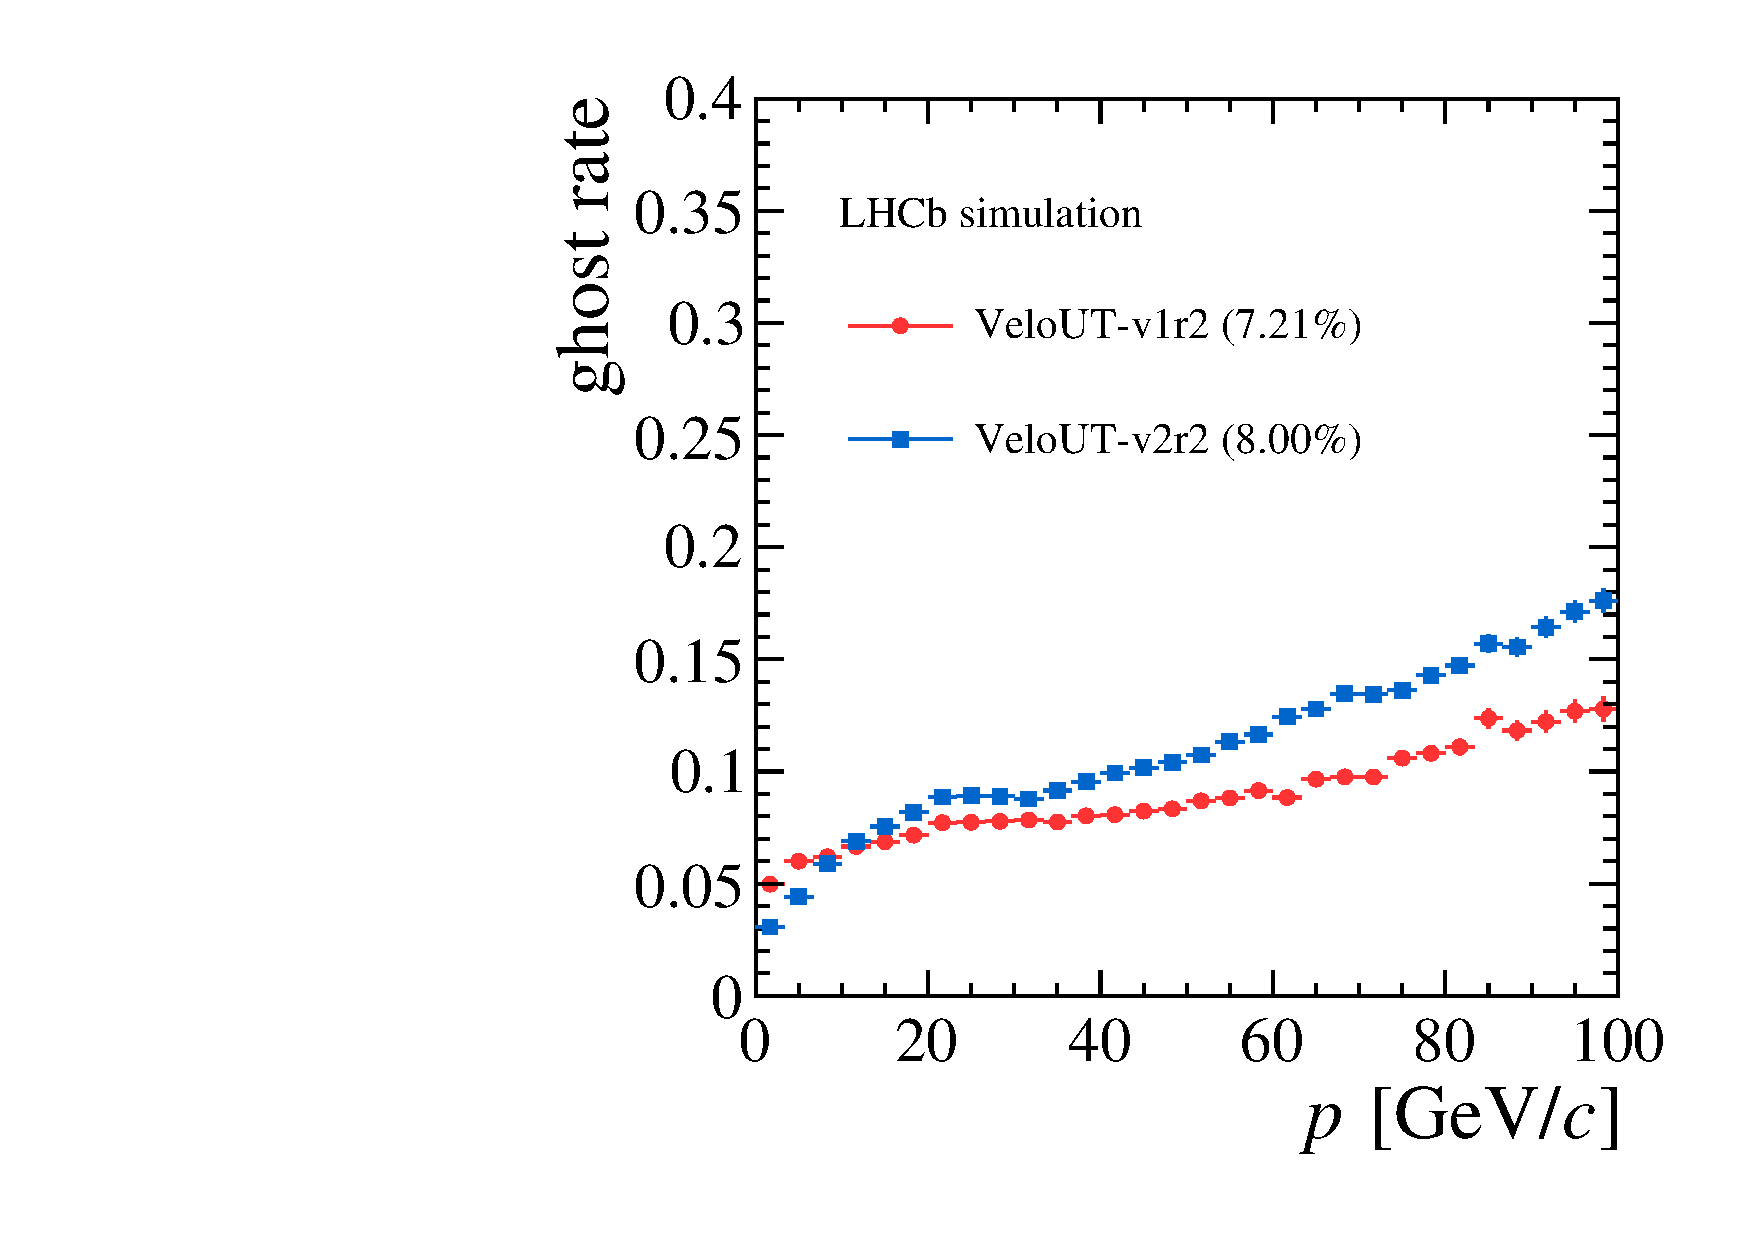
\includegraphics[width=0.45\textwidth]{figs/upstream-tracking-upgrade/gr_p_comp.pdf}
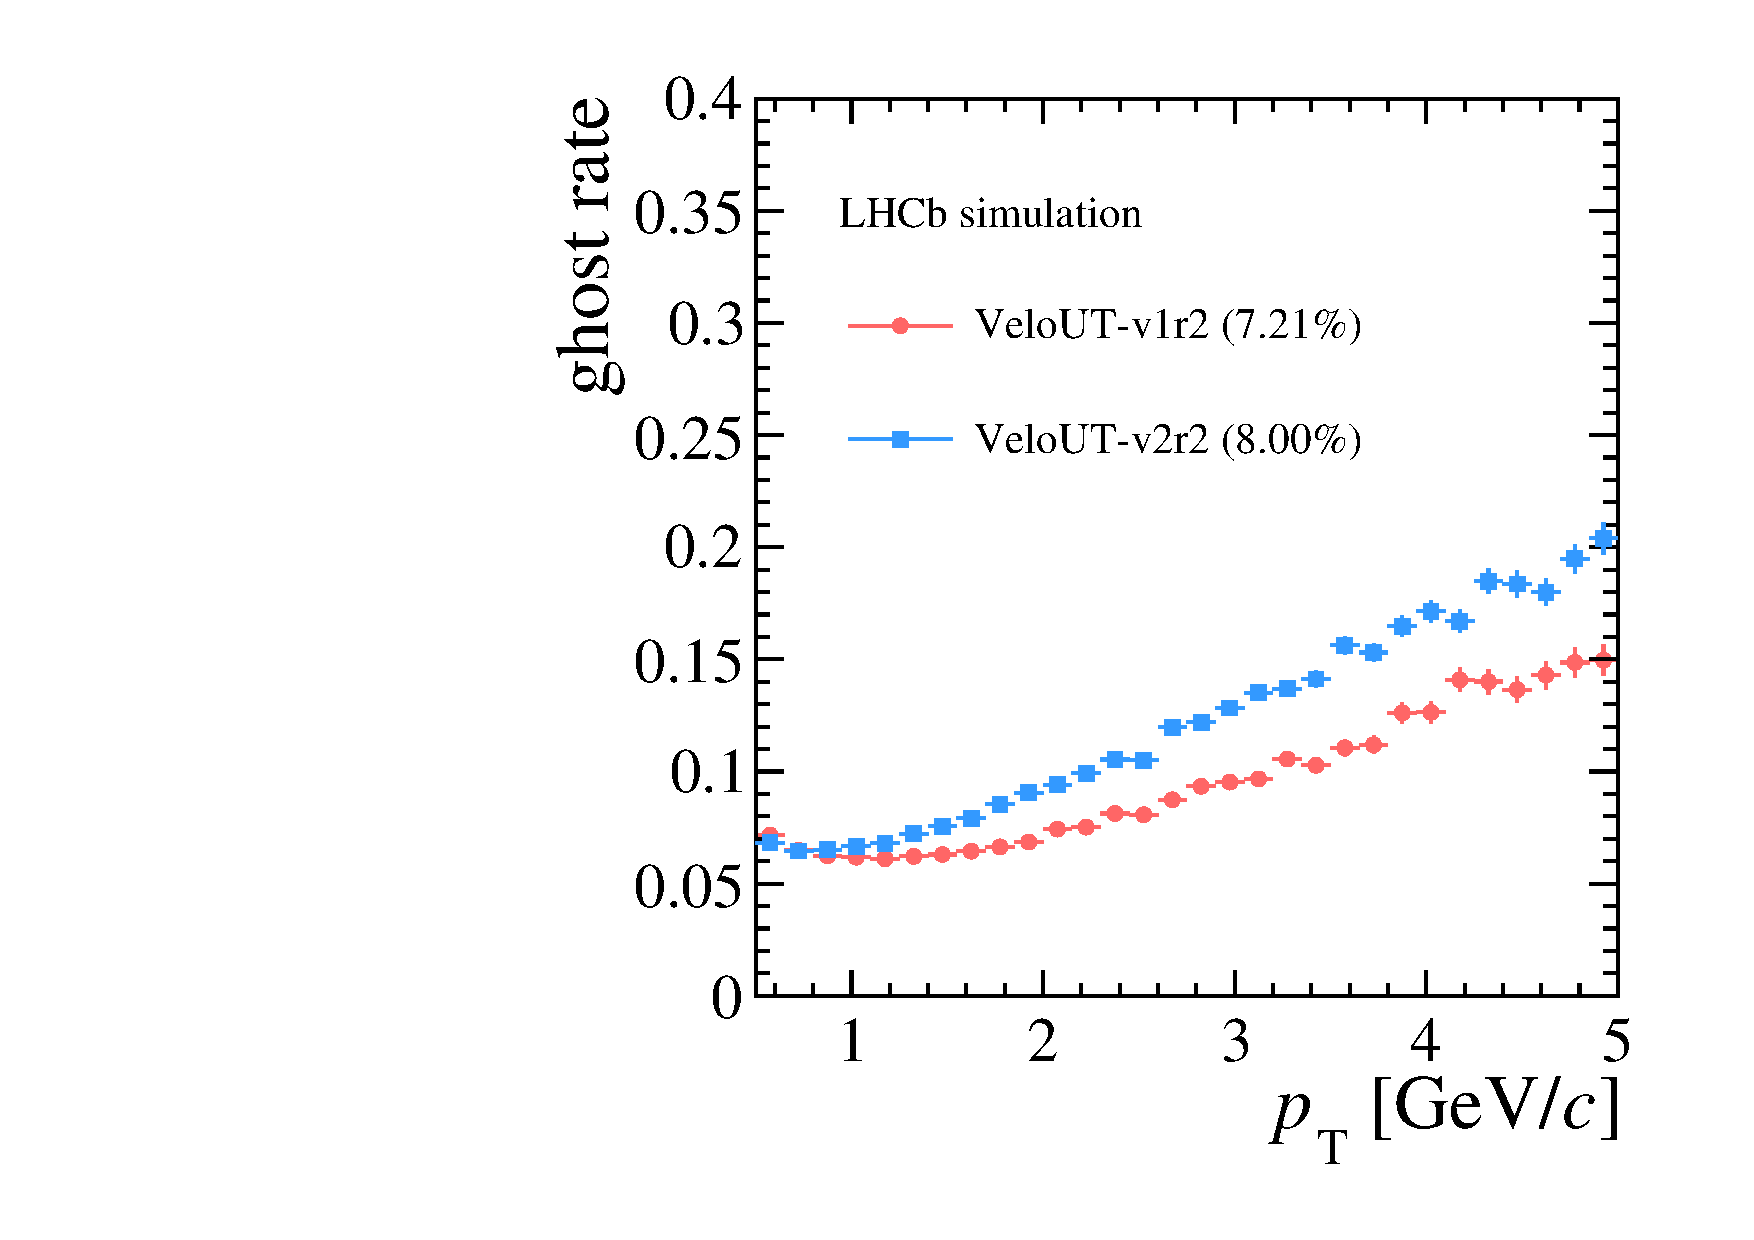
\includegraphics[width=0.45\textwidth]{figs/upstream-tracking-upgrade/gr_pt_comp.pdf}
\caption{The ghost rate as a function of \ptot and \pt for both the initial version (\texttt{v1r2}) and the optimised version (\texttt{v2r2}) of the \velout algorithm.}
\label{fig:gr_velout_comp}
\end{figure}

\subsubsection{Forward}

The track reconstruction efficiency, ghost rate and execution time of the Forward algorithm using \velo or \velout tracks as input are shown in Table~\ref{tab:perf_forward_comp}. The track reconstruction efficiency as a function of \ptot and \pt are shown in Fig.~\ref{fig:eff_fwd_comp}. The ghost rate as a function of \ptot and \pt are shown in Fig.~\ref{fig:gr_fwd_comp}. The use of \velout tracks as input to the Forward algorithm drastically reduces the ghost rate and execution time. This comes at a small cost in the track reconstruction efficiency.

\begin{table}[!tb]
\caption{The performances of the Forward algorithm using \velo or \velout tracks as input in terms of track reconstruction efficiency, ghost rate and execution time.}
\resizebox{\columnwidth}{!}{
\begin{tabular}{c|c|c|c|c}
    & Efficiency [\%] & Ghost rate [\%] & VeloUT [ms] & Forward [ms] \\
   \hline
   Velo-Forward  & 94.10  & 41.55  &  -  & 18.28 \\
   VeloUT-Forward  & 93.37  & 14.08  &  0.81 & \hphantom{0}3.45  \\
 \end{tabular}
 }
 \label{tab:perf_forward_comp}
\end{table}

\begin{figure}[!tb]
\centering
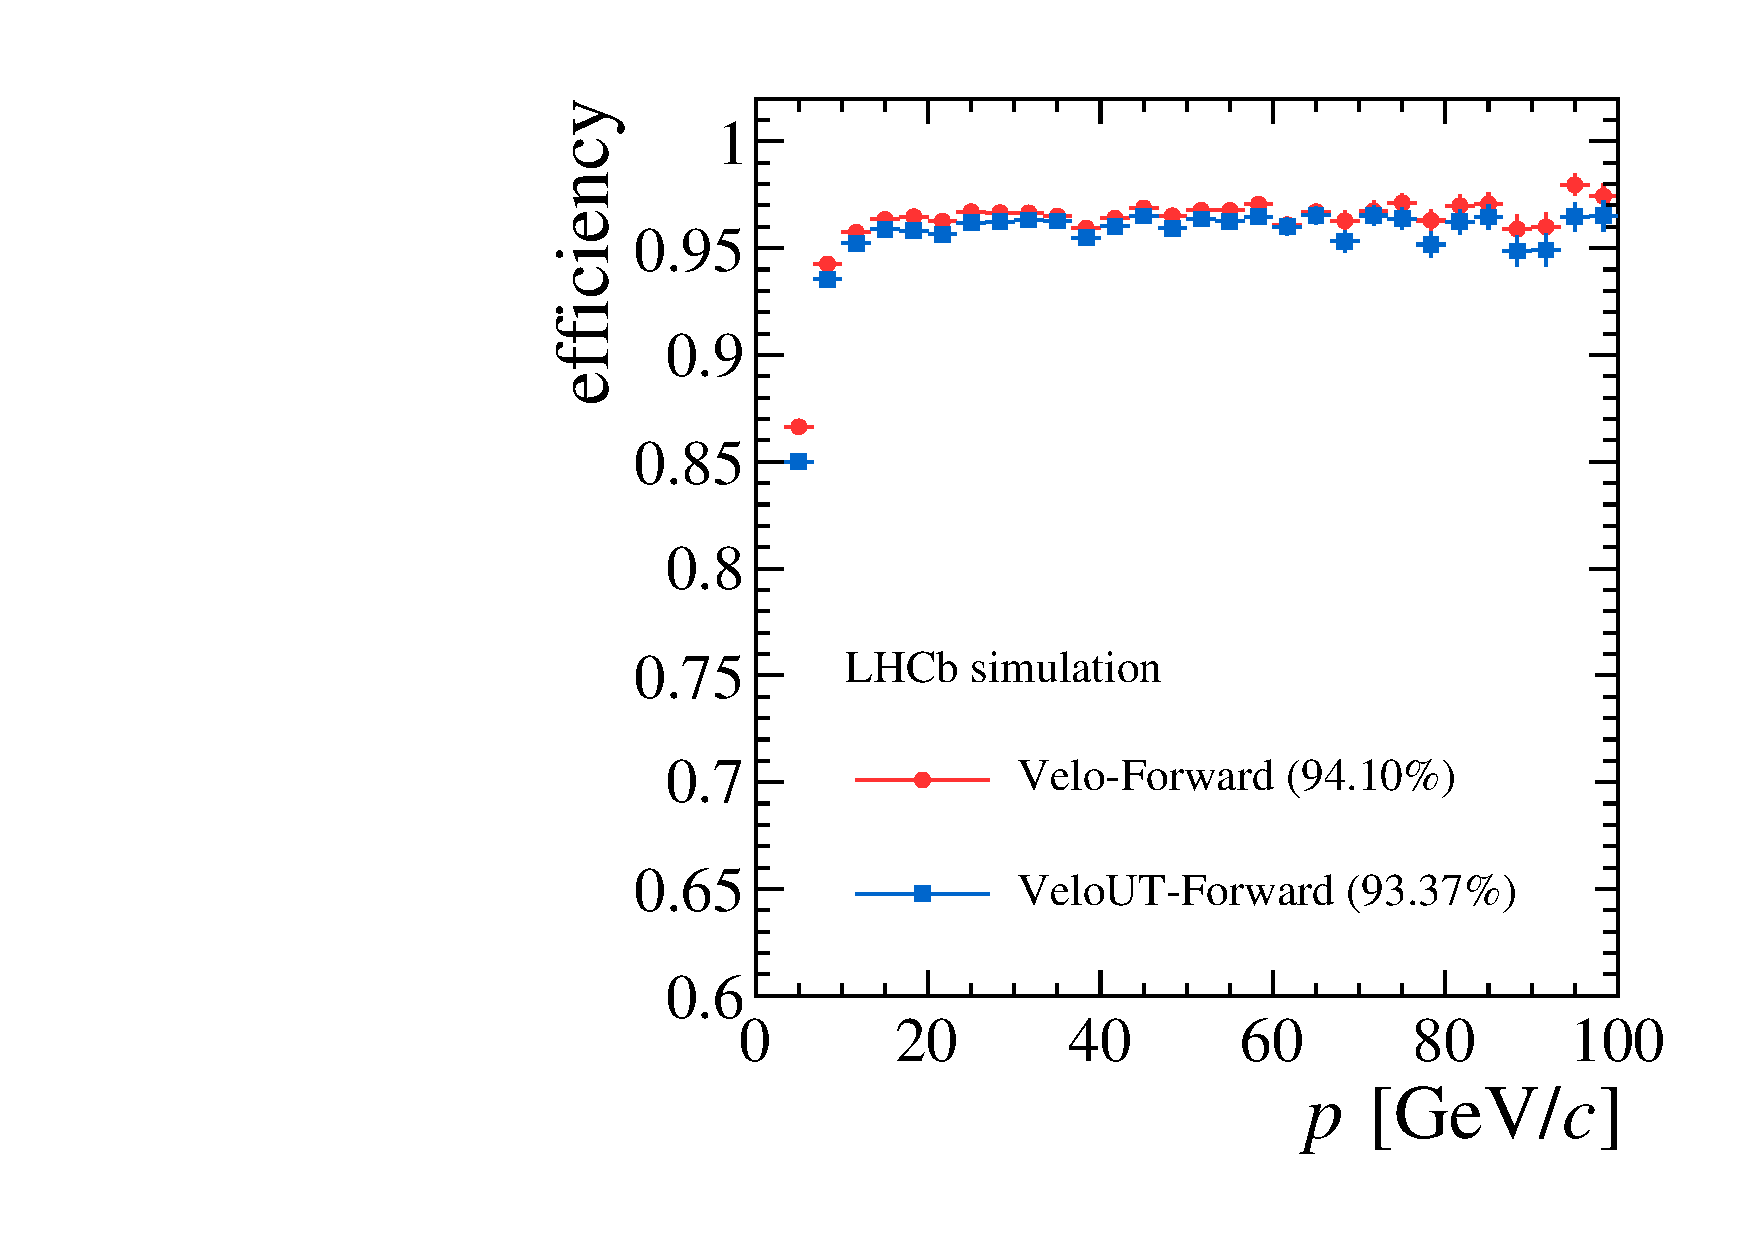
\includegraphics[width=0.45\textwidth]{figs/upstream-tracking-upgrade/fwd_eff_p_comp.pdf}
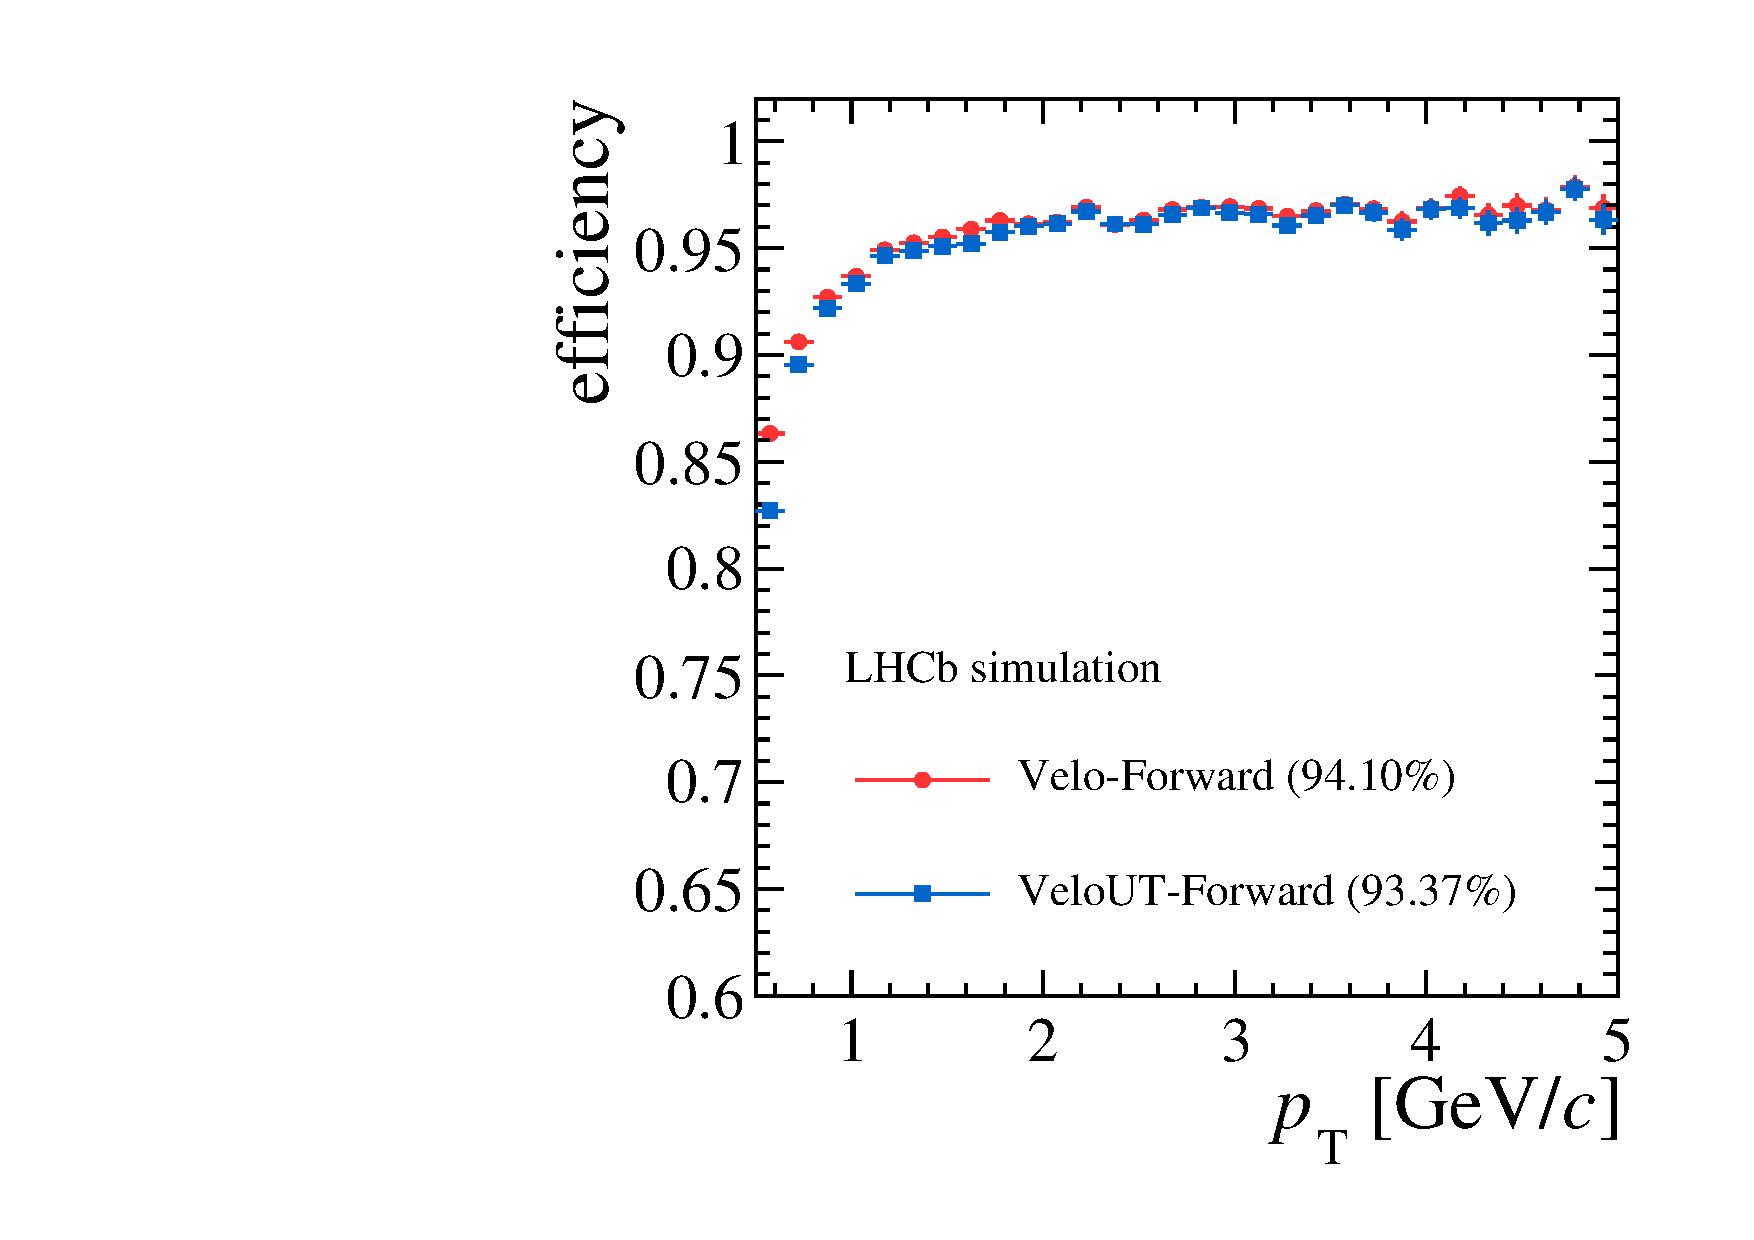
\includegraphics[width=0.45\textwidth]{figs/upstream-tracking-upgrade/fwd_eff_pt_comp.pdf}
\caption{The track reconstruction efficiency of the Forward algorithm using \velo or \velout tracks as a function of \ptot and \pt.}
\label{fig:eff_fwd_comp}
\end{figure}

\begin{figure}[!tb]
\centering
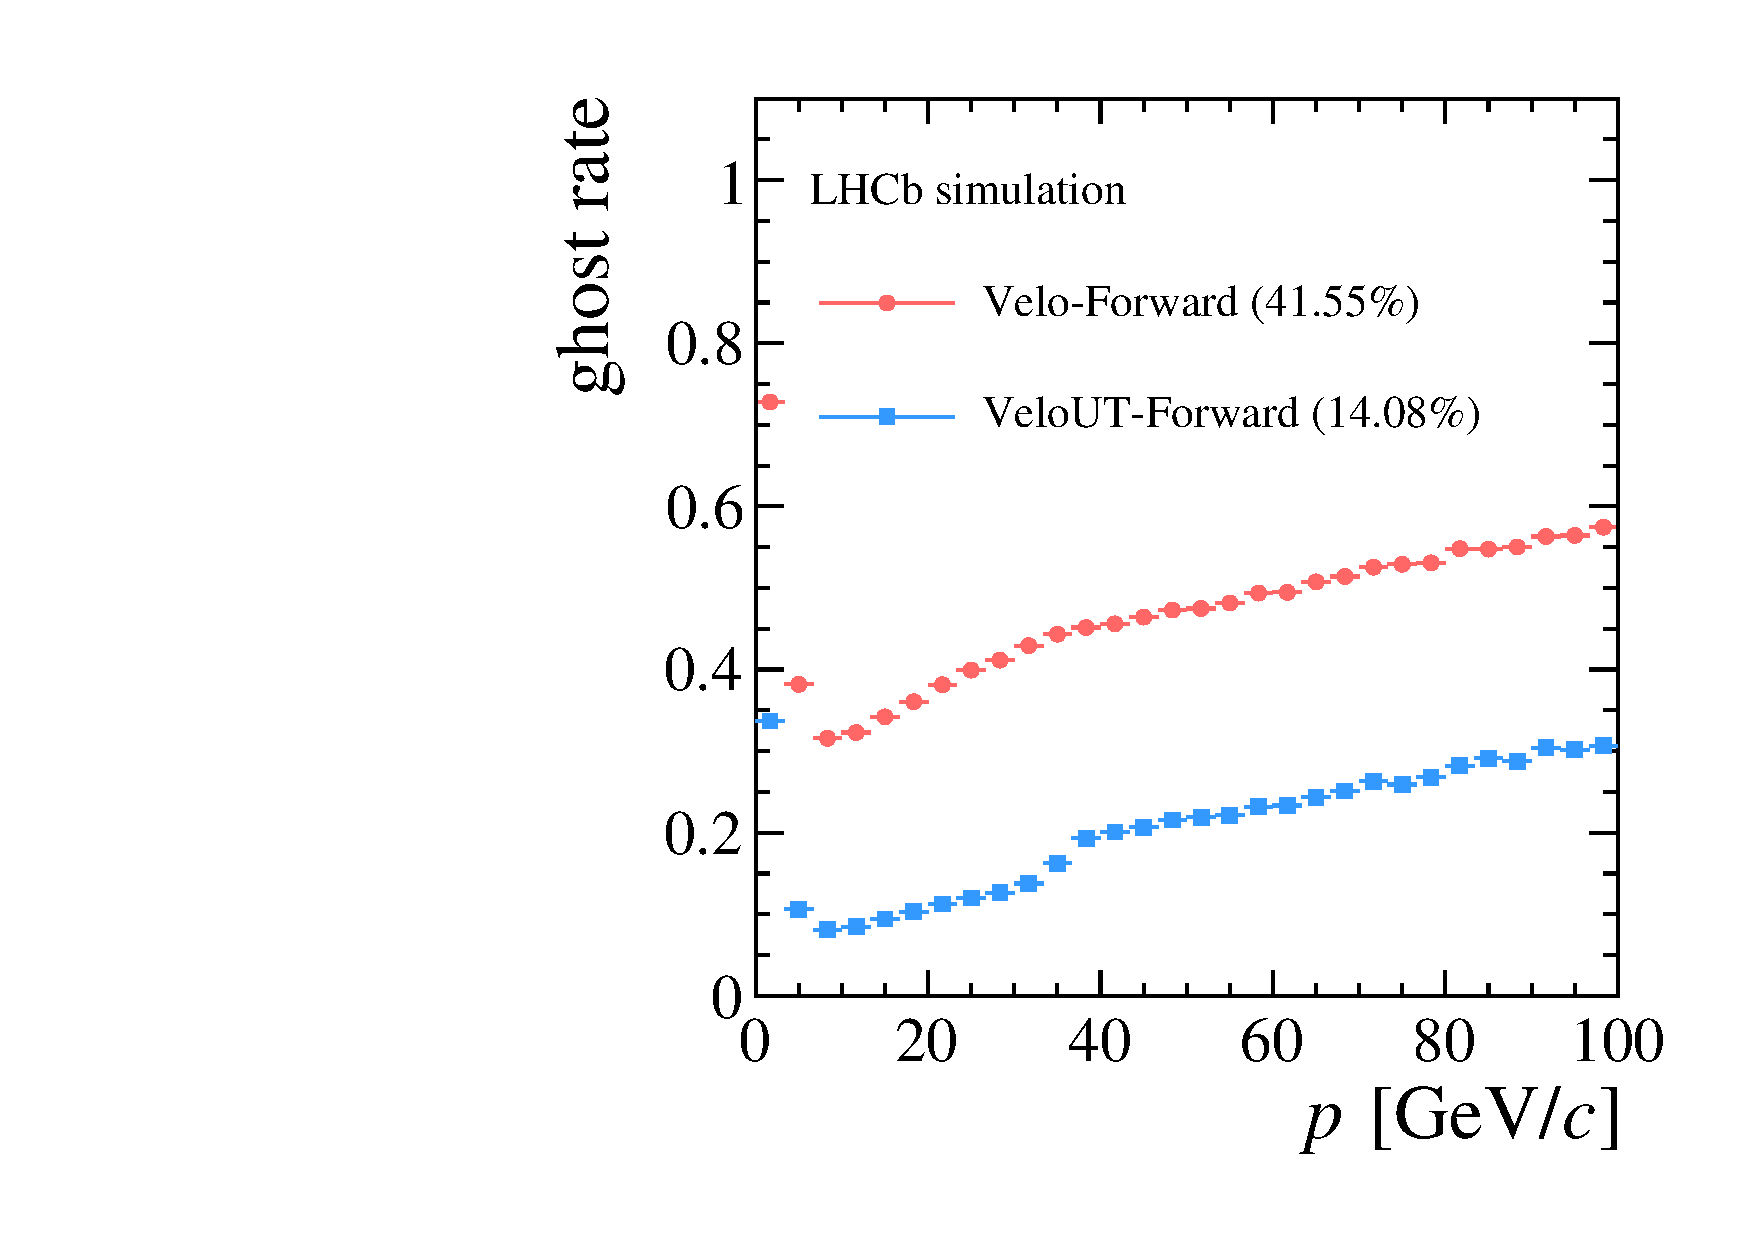
\includegraphics[width=0.45\textwidth]{figs/upstream-tracking-upgrade/fwd_gr_p_comp.pdf}
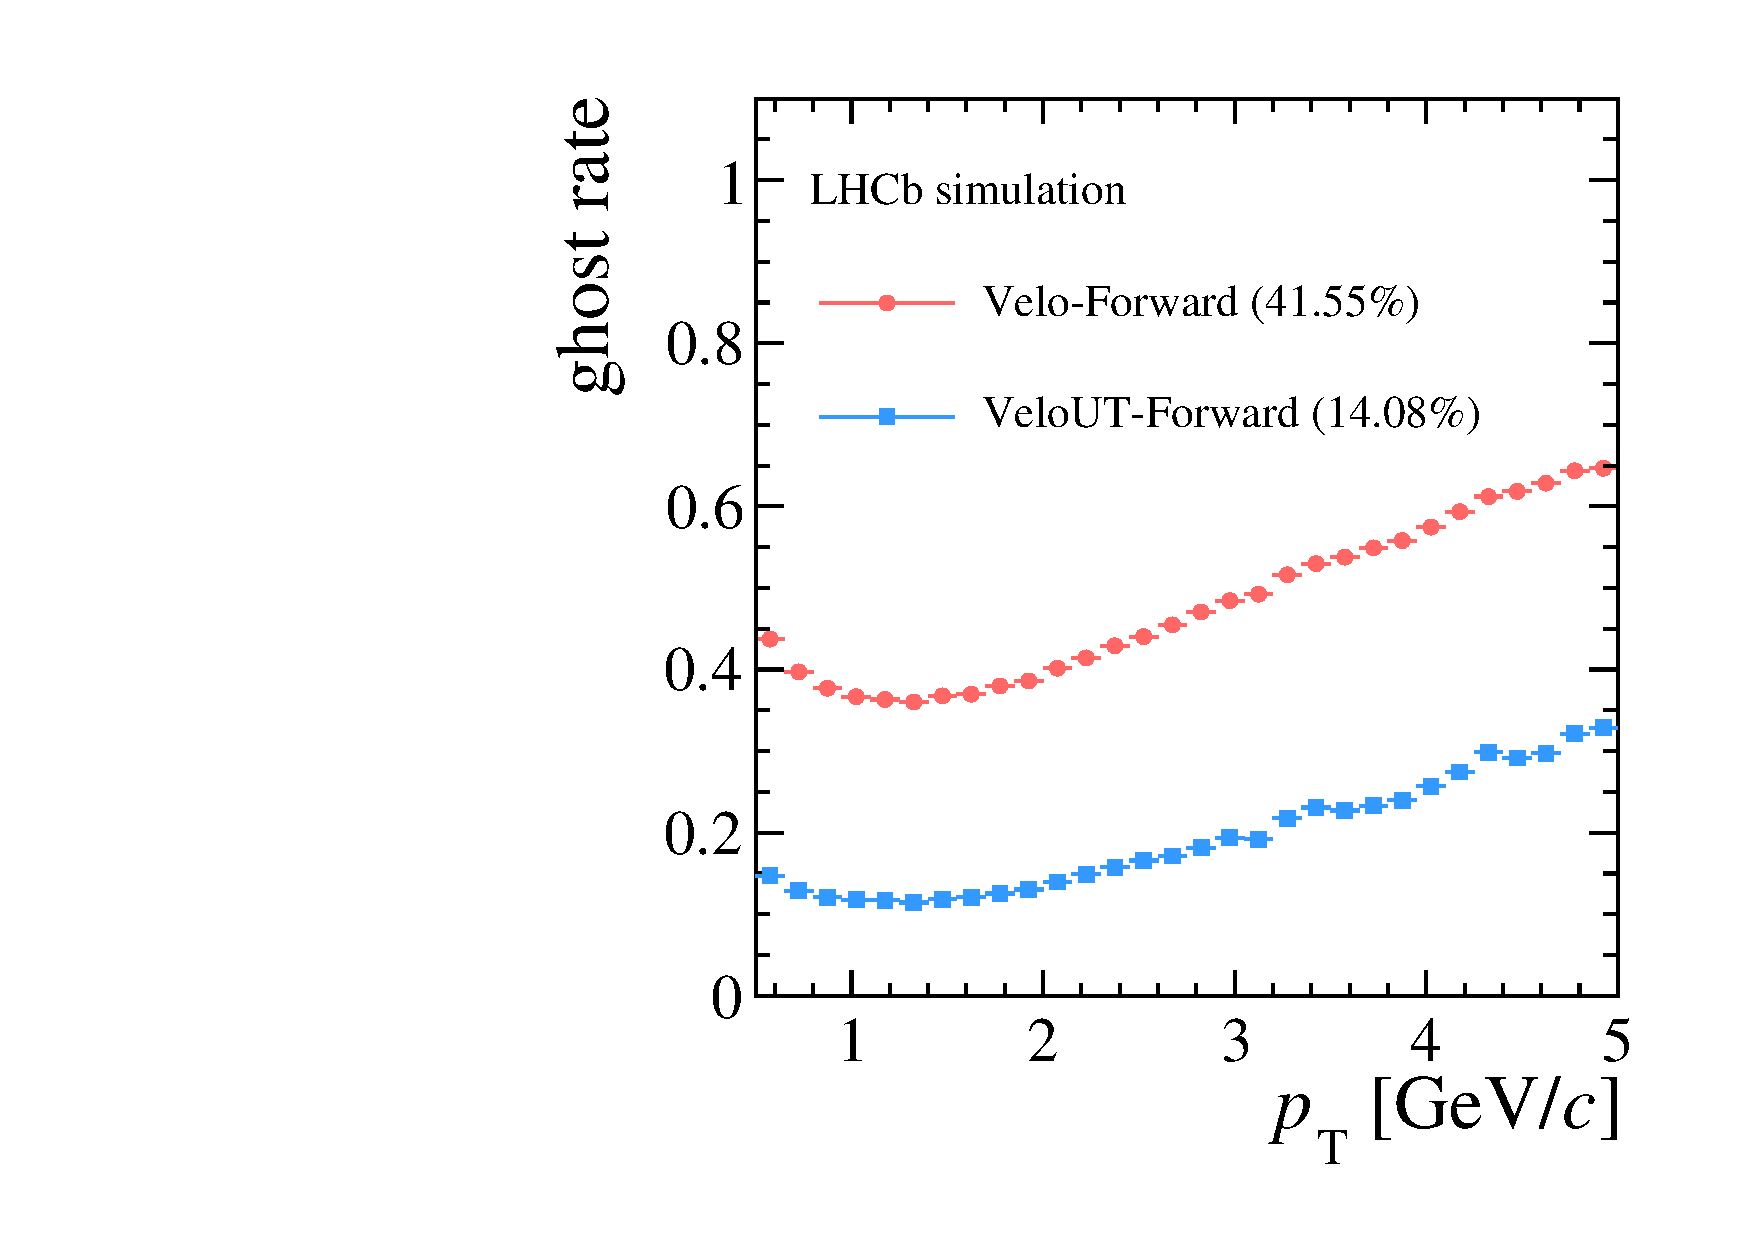
\includegraphics[width=0.45\textwidth]{figs/upstream-tracking-upgrade/fwd_gr_pt_comp.pdf}
\caption{The ghost rate of the Forward algorithm using \velo or \velout tracks as a function of \ptot and \pt.}
\label{fig:gr_fwd_comp}
\end{figure}

\subsection{Summary}

The majority of \lhcb analyses use long tracks, which traverse the full tracking detector. These tracks will be reconstructed by the Forward tracking algorithm at the software trigger level in the \lhcb upgrade. Previously, \velo tracks were used as input to the Forward algorithm. However, a novel method was investigated to use upstream tracks, reconstructed by the \velout algorithm, as input. The vast improvements in the performance of the \velout algorithm and the subsequent improvement to the overall tracking sequence led to the algorithm being adopted into the default tracking sequence for the \lhcb Upgrade~\cite{upgrade-trigger-tdr,upgrade-tracker-tdr}. It will play a large role in allowing \lhcb to become the first hadron collider experiment to operate a software-only trigger at the full event rate.

